\documentclass[11pt,a4paper]{article}

% ---------- Page / font ----------
\usepackage[a4paper,margin=1in]{geometry}
\usepackage[T1]{fontenc}
\usepackage{lmodern}
\usepackage{microtype}
\usepackage{algorithm}
\usepackage{algpseudocode} % algorithmicx

% ---------- Math ----------
\usepackage{amsmath,amssymb,amsthm,bm,mathtools}
\numberwithin{equation}{section}
\numberwithin{figure}{section}
\numberwithin{table}{section}

% ---------- Figures / tables ----------
\usepackage{graphicx}
\graphicspath{{../}}
\usepackage{subcaption}
\usepackage{float}        % allows [H] to control float placement
\usepackage{booktabs}     % professional tables
\usepackage{array}
\usepackage{tabularx}
\usepackage{siunitx}


% ---------- Algorithms (KEEP from first preamble) ----------
\usepackage{algorithm}
\usepackage{algpseudocode}

% ---------- Hyperlinks & references ----------
\usepackage[hidelinks]{hyperref}
\usepackage[nameinlink,capitalise]{cleveref}

% ---------- Captions ----------
\usepackage{caption}
\captionsetup{font=small}

% ---------- Theorems ----------
\newtheorem{theorem}{Theorem}
\newtheorem{proposition}{Proposition}
\newtheorem{lemma}{Lemma}
\newtheorem{assumption}{Assumption}
\theoremstyle{definition}
\newtheorem{definition}{Definition}
\newtheorem{remark}{Remark}

% ---------- Notation helpers ----------
\newcommand{\R}{\mathbb{R}}
\newcommand{\norm}[1]{\left\lVert #1 \right\rVert}
\newcommand{\ip}[2]{\left\langle #1, #2 \right\rangle}
\newcommand{\argmin}{\operatorname*{arg\,min}}
\newcommand{\proj}{\operatorname{proj}}
\newcommand{\diag}{\operatorname{diag}}
\newcommand{\E}{\mathbb{E}}
\newcommand{\pos}[1]{\left[#1\right]_+}

% ---------- Title ----------
\title{Augmented Lagrangian Constraint Handling in CMA-ES with Experiments}
\author{Fangdu REN, Tanguy Villain, Xiangyu LUO}
\date{}
\begin{document}

\maketitle

\begin{abstract}
This report presents a comprehensive analysis of the Augmented Lagrangian CMA-ES (AL-CMA-ES), a standard framework for handling constraints in black-box optimization without the ill-conditioning issues inherent in static penalty methods. We review the theoretical foundations of the augmented Lagrangian method and detail its integration into the CMA-ES evolutionary loop, focusing on the interplay between covariance adaptation and the adaptive updates of Lagrange multipliers and penalty coefficients. Through numerical experiments on linearly constrained, ill-conditioned, and non-smooth benchmarks, we evaluate the algorithm's convergence behavior and compare its performance against standard penalty-based approaches. The results demonstrate that AL-CMA-ES effectively decouples feasibility enforcement from landscape conditioning, offering a robust and sample-efficient solution for continuous constrained optimization problems.
\end{abstract}

\tableofcontents
\newpage

%========================================================
%\section{Introduction}\label{sec:introduction}


%========================================================
\section{Augmented Lagrangian Method}\label{sec:al}
This section introduces the augmented Lagrangian (AL) method for constrained optimization by building up from the standard Lagrangian and penalty formulations. We first formalize the constrained problem and common feasibility measures, then present the AL construction, and finally use simple comparisons to clarify why augmentation is often necessary and how it reshapes the merit function.

\subsection{Constrained problem and feasibility measures}\label{subsec:al-setting}
We consider constrained optimization problems of the form
\begin{equation}
\label{eq:constrained-problem}
  \min_{\bm{x}\in \R^n} f(\bm{x})
  \quad\text{s.t.}\quad
  g_i(\bm{x}) \le 0,\ i=1,\dots,m,
  \qquad
  h_j(\bm{x}) = 0,\ j=1,\dots,p,
\end{equation}
where $f:\R^n\to\R$ is the objective function and $g_i,h_j:\R^n\to\R$ encode inequality and equality constraints, respectively. The feasible set is
\(
\mathcal{F}:=\{\bm{x}\in\R^n:\ g_i(\bm{x})\le 0\ \forall i,\ h_j(\bm{x})=0\ \forall j\}.
\)
In black-box optimization, evaluations of $f(\bm{x})$ and $g_i(\bm{x}),h_j(\bm{x})$ are available (e.g., via simulation), while gradients may be unavailable or unreliable. This setting motivates constraint handling mechanisms that transform~\eqref{eq:constrained-problem} into an unconstrained \emph{merit function} that can be optimized by derivative-free methods, while still steering the search toward feasibility.

For compactness, we collect constraints as
\begin{equation}
  \begin{aligned}
    g(\bm{x}) &:= (g_1(\bm{x}),\dots,g_m(\bm{x}))^\top,\\
    h(\bm{x}) &:= (h_1(\bm{x}),\dots,h_p(\bm{x}))^\top.
  \end{aligned}
\end{equation}
For inequalities, we denote the componentwise positive part by $\pos{\cdot}$, i.e., $\pos{a}=\max(0,a)$ and $\pos{g(\bm{x})}$ applies this operation to each component of $g(\bm{x})$. A common scalar measure of infeasibility is then, for example,
\(
V(\bm{x}) := \norm{\pos{g(\bm{x})}}_2
\)
or $\sum_{i=1}^m \pos{g_i(\bm{x})}$.
We also call a constraint $g_i$ \emph{active} at $\bm{x}$ if $g_i(\bm{x})=0$.\cite{DufosseHansen}
Equality constraints can be handled directly (e.g., via squared penalties) or rewritten as inequalities using a numerical tolerance, for example $\pos{|h_j(\bm{x})|-\varepsilon}\le 0$ with $\varepsilon\ge 0$.\cite{DufosseHansen,Atamna2016}

Our overall goal is to design a merit function that remains meaningful for black-box optimization: it should encourage feasibility, avoid pathological scaling, and provide stable behavior even when the associated unconstrained subproblem is solved only approximately.

\subsection{Standard Lagrangian and penalty methods}\label{subsec:al-lag-pen}
The \emph{standard Lagrangian} associated with~\eqref{eq:constrained-problem} is
\begin{equation}
\label{eq:lagrangian}
  \mathcal{L}(\bm{x},\bm{\lambda},\bm{\nu})
  := f(\bm{x}) + \bm{\lambda}^\top g(\bm{x}) + \bm{\nu}^\top h(\bm{x}),
  \qquad \bm{\lambda}\in\R^m,\ \bm{\nu}\in\R^p,
\end{equation}
with the convention that inequality multipliers satisfy $\bm{\lambda}\ge 0$ componentwise. The key idea is to \emph{relax} the constraints into the objective through the multipliers: for a fixed $(\bm{\lambda},\bm{\nu})$, minimizing $\mathcal{L}(\cdot,\bm{\lambda},\bm{\nu})$ encourages constraint satisfaction when multipliers are large.

Under standard regularity conditions, first-order optimality of~\eqref{eq:constrained-problem} is characterized by the Karush--Kuhn--Tucker (KKT) conditions: there exist multipliers $(\bm{\lambda}^\star,\bm{\nu}^\star)$ such that
\begin{align}
  \nabla f(\bm{x}^\star) + \nabla g(\bm{x}^\star)^\top \bm{\lambda}^\star + \nabla h(\bm{x}^\star)^\top \bm{\nu}^\star &= \bm{0},
  \label{eq:kkt-stationarity}\\
  g(\bm{x}^\star)\le \bm{0},\quad h(\bm{x}^\star)=\bm{0},\quad \bm{\lambda}^\star\ge \bm{0},\quad \bm{\lambda}^\star\odot g(\bm{x}^\star) &= \bm{0}.
  \label{eq:kkt-feas}
\end{align}
In convex problems, the Lagrangian also underpins duality theory; however, in nonconvex and black-box settings we mainly use~\eqref{eq:lagrangian} as a design principle to build scalar merit functions and multiplier update rules.\cite{NocedalWright}

Penalty functions provide an alternative to the Lagrangian by directly penalizing constraint violations. A broad family of penalty merit functions takes the form\cite{DufosseHansen}
\begin{equation}
\label{eq:general-penalty}
  P_\alpha(\bm{x},\bm{c})
  := f(\bm{x}) + \sum_{i=1}^m c_i\,\pos{g_i(\bm{x})}^{\alpha},
  \qquad \alpha\in\{1,2\},\ \bm{c}>\bm{0}.
\end{equation}
The case $\alpha=1$ yields a \emph{linear} penalty (potentially exact but non-smooth at the boundary), while $\alpha=2$ yields a smooth \emph{quadratic} penalty.
The classical quadratic penalty method for equalities can be seen as a special case of~\eqref{eq:general-penalty} applied to $h$:
\begin{equation}
\label{eq:quadratic-penalty}
  Q_\rho(\bm{x})
  := f(\bm{x})
  + \frac{\rho}{2}\norm{h(\bm{x})}^2
  + \frac{\rho}{2}\norm{\pos{g(\bm{x})}}^2,
  \qquad \rho>0,
\end{equation}
where $\rho$ is the penalty parameter (or penalty coefficient). As $\rho\to\infty$, minimizers of $Q_\rho$ can approach feasibility under appropriate conditions, but this comes with a major drawback: large $\rho$ typically induces severe \emph{ill-conditioning} of the penalized landscape.\cite{NocedalWright} Intuitively, the penalty term creates narrow valleys around the feasible set; consequently, the inner minimization becomes progressively harder as $\rho$ increases, and algorithms can require very small steps (or very fine covariance adaptation) to make progress.

The main practical drawback of penalty methods is that they involve \emph{tuning} the penalty coefficients $\bm{c}$ (or $\rho$). In particular, quadratic penalties typically require large coefficients on active constraints to drive the minimizer into the feasible region, which in turn can create ill-conditioned landscapes and slow down the inner optimizer.\cite{NocedalWright,DufosseHansen} Linear penalties avoid ill-conditioning but sacrifice smoothness; moreover, exactness requires $c_i$ to be at least as large as the (unknown) optimal multiplier $\lambda_i^\star$ for each active constraint.\cite{DufosseHansen}

These considerations motivate the augmented Lagrangian method, which combines multiplier information with moderated quadratic penalties to obtain stronger feasibility control without requiring extreme penalty growth.\cite{NocedalWright}

\subsection{Augmented Lagrangian method}\label{subsec:al-method}
The augmented Lagrangian (AL) method---also known as the \emph{method of multipliers}---combines the Lagrangian idea with a quadratic penalty to achieve both feasibility pressure and meaningful multiplier estimates.\cite{NocedalWright}
For equality constraints $h(\bm{x})=\bm{0}$, the classical augmented Lagrangian reads
\begin{equation}
\label{eq:al-equality}
  \mathcal{L}_\rho(\bm{x},\bm{\nu})
  := f(\bm{x}) + \bm{\nu}^\top h(\bm{x}) + \frac{\rho}{2}\norm{h(\bm{x})}^2.
\end{equation}
Compared to the pure quadratic penalty, the linear term $\bm{\nu}^\top h(\bm{x})$ acts as a correction that steers stationary points of the penalized subproblems toward KKT points without requiring $\rho\to\infty$.

For inequality constraints, a common construction introduces a multiplier $\lambda_i\ge 0$ and penalty coefficient $\rho_i>0$ per constraint.\cite{Atamna2016,DufosseHansen} The corresponding AL function can be written in a compact ``positive-part'' form,
\begin{equation}
\label{eq:al-inequality-prox}
  H(\bm{x},\bm{\lambda},\bm{\rho})
  := f(\bm{x})
  + \frac{1}{2}\sum_{i=1}^m \rho_i\, \pos{g_i(\bm{x}) + \lambda_i/\rho_i}^{\,2}
  - \frac{1}{2}\sum_{i=1}^m \frac{\lambda_i^2}{\rho_i},
  \qquad \bm{\lambda}\ge \bm{0},\ \bm{\rho}>\bm{0},
\end{equation}
which is equivalent (per constraint) to the piecewise definition
\begin{equation}
\label{eq:al-inequality-piecewise}
  H_i(\bm{x})
  =
  \begin{cases}
    \lambda_i g_i(\bm{x}) + \frac{\rho_i}{2}\, g_i(\bm{x})^2, & \lambda_i + \rho_i g_i(\bm{x}) \ge 0,\\[2mm]
    -\dfrac{\lambda_i^2}{2\rho_i}, & \lambda_i + \rho_i g_i(\bm{x}) < 0.
  \end{cases}
\end{equation}
The second branch is constant in $\bm{x}$; hence, once constraint $i$ is sufficiently satisfied (roughly $g_i(\bm{x})<-\lambda_i/\rho_i$), it stops influencing the search. Moreover, if $g_i$ is differentiable, $H_i$ is continuously differentiable because the derivative of the first branch w.r.t.\ $g_i$ equals $\lambda_i+\rho_i g_i$, which vanishes at the switching point.\cite{DufosseHansen}

This formulation subsumes quadratic penalties. Setting $\bm{\lambda}=\bm{0}$ in~\eqref{eq:al-inequality-prox} yields
\(
H(\bm{x},\bm{0},\bm{\rho}) = f(\bm{x}) + \frac{1}{2}\sum_i \rho_i\,\pos{g_i(\bm{x})}^2,
\)
which corresponds to a quadratic penalty with coefficients $c_i=\rho_i/2$.\cite{DufosseHansen} From this perspective, AL can be seen as ``quadratic penalty + adaptive linear correction'' via the multipliers.

Augmented Lagrangian methods are typically implemented with an outer loop on $(\bm{\lambda},\bm{\rho})$. Each outer iteration carries out an inner minimization on $\bm{x}$:
\par

\begin{algorithm}[H]
\caption{AL outer loop (inequality constraints)}
\label{alg:alm}
\begin{algorithmic}[1]

\Require Initial $\bm{x}^{(0)}$, $\bm{\lambda}^{(0)} \ge \bm{0}$, $\bm{\rho}^{(0)} > \bm{0}$

\For{$t = 0,1,2,\dots$ until termination}

\State $\bm{x}^{(t+1)} \gets 
\arg\min_{\bm{x}} H(\bm{x},\bm{\lambda}^{(t)},\bm{\rho}^{(t)})$ (approximately)

\State $\bm{\lambda}^{(t+1)} \gets 
\pos{\bm{\lambda}^{(t)} + \bm{\rho}^{(t)} \odot g(\bm{x}^{(t+1)})}$

\If{violation reduction is insufficient}
    \State $\bm{\rho}^{(t+1)} \gets \tau\,\bm{\rho}^{(t)}$ \Comment{$\tau > 1$}
\Else
    \State $\bm{\rho}^{(t+1)} \gets \bm{\rho}^{(t)}$
\EndIf

\EndFor

\end{algorithmic}
\end{algorithm}

The key practical feature is that $\bm{\rho}$ is increased only when needed; ideally, multipliers approach KKT values while penalty coefficients remain moderate, preventing ill-conditioning.\cite{NocedalWright}
In black-box settings, the inner minimization can be carried out by any suitable unconstrained optimizer, and the outer updates are driven by the constraint values observed at the current incumbent iterate.

\subsection{Why augmentation matters}\label{subsec:al-limitations}
Having introduced the standard Lagrangian and penalty formulations as well as the augmented Lagrangian construction, we now use simple examples to clarify why augmentation is often necessary in practice. The standard Lagrangian and simple penalty approaches highlight complementary weaknesses that become acute in nonconvex black-box settings. A typical Lagrangian dual-ascent scheme alternates between approximately minimizing $\mathcal{L}(\bm{x},\bm{\lambda},\bm{\nu})$ and updating multipliers based on constraint violations. Such updates can oscillate around the feasible set and provide weak feasibility pressure when multipliers are far from their KKT values. Penalty methods enforce feasibility more directly, but quadratic penalties often require large coefficients that create narrow valleys around the constraint manifold and make the inner minimization progressively harder; linear penalties avoid this ill-conditioning at the expense of non-smoothness and still require coefficients comparable to unknown optimal multipliers.\cite{NocedalWright,DufosseHansen} Finally, in nonconvex problems, objective reduction can be dominated by attractive infeasible basins, so progress in $f$ alone is not a reliable indicator of progress toward a feasible solution.

To illustrate these behaviors in a controlled setting, we consider two low-dimensional equality-constrained problems and compare a basic dual-ascent Lagrangian scheme with an augmented Lagrangian method.

\subsubsection{Case A: convex quadratic program}\label{subsubsec:case-a}
We consider the equality-constrained quadratic program
\begin{equation}
  \label{eq:case-a}
  \begin{aligned}
    \min_{(x_1,x_2)\in\R^2}\quad & (x_1-2)^2 + (x_2-1)^2,\\
    \text{s.t.}\quad & x_1 + x_2 = 1.
  \end{aligned}
\end{equation}
The constrained optimum is $\bm{x}^\star=(1,0)$ with $f^\star=2$.

\Cref{fig:case-a-trajectory} visualizes the iterates in the $(x_1,x_2)$ plane. From the same initialization, the augmented approach moves quickly toward feasibility and then progresses along the constraint toward the constrained minimizer.

\begin{figure}[H]
  \centering
  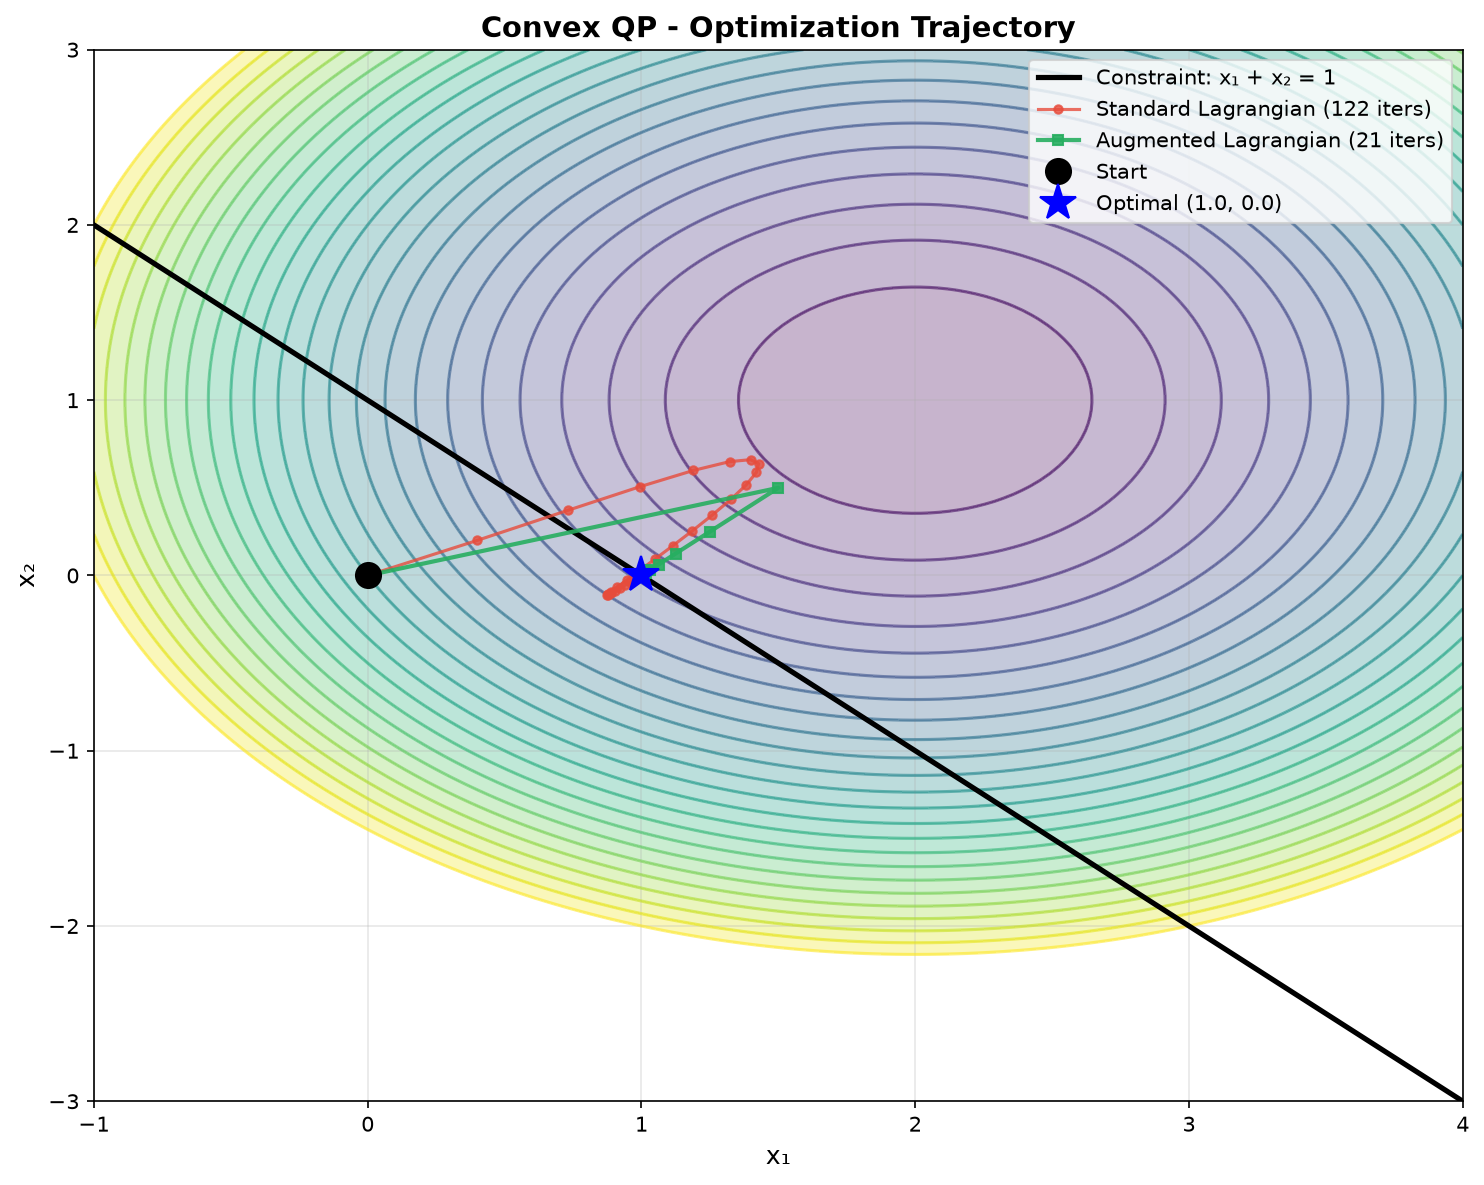
\includegraphics[width=0.75\linewidth]{results/lagrangian_comparison/case_a_convex/01_trajectory.png}
  \caption{Case A: trajectories.}
  \label{fig:case-a-trajectory}
\end{figure}

\Cref{fig:case-a-convergence} shows that both methods converge to the feasible optimum, but the augmented approach reaches the stopping criterion with substantially fewer outer iterations.

\begin{figure}[H]
  \centering
  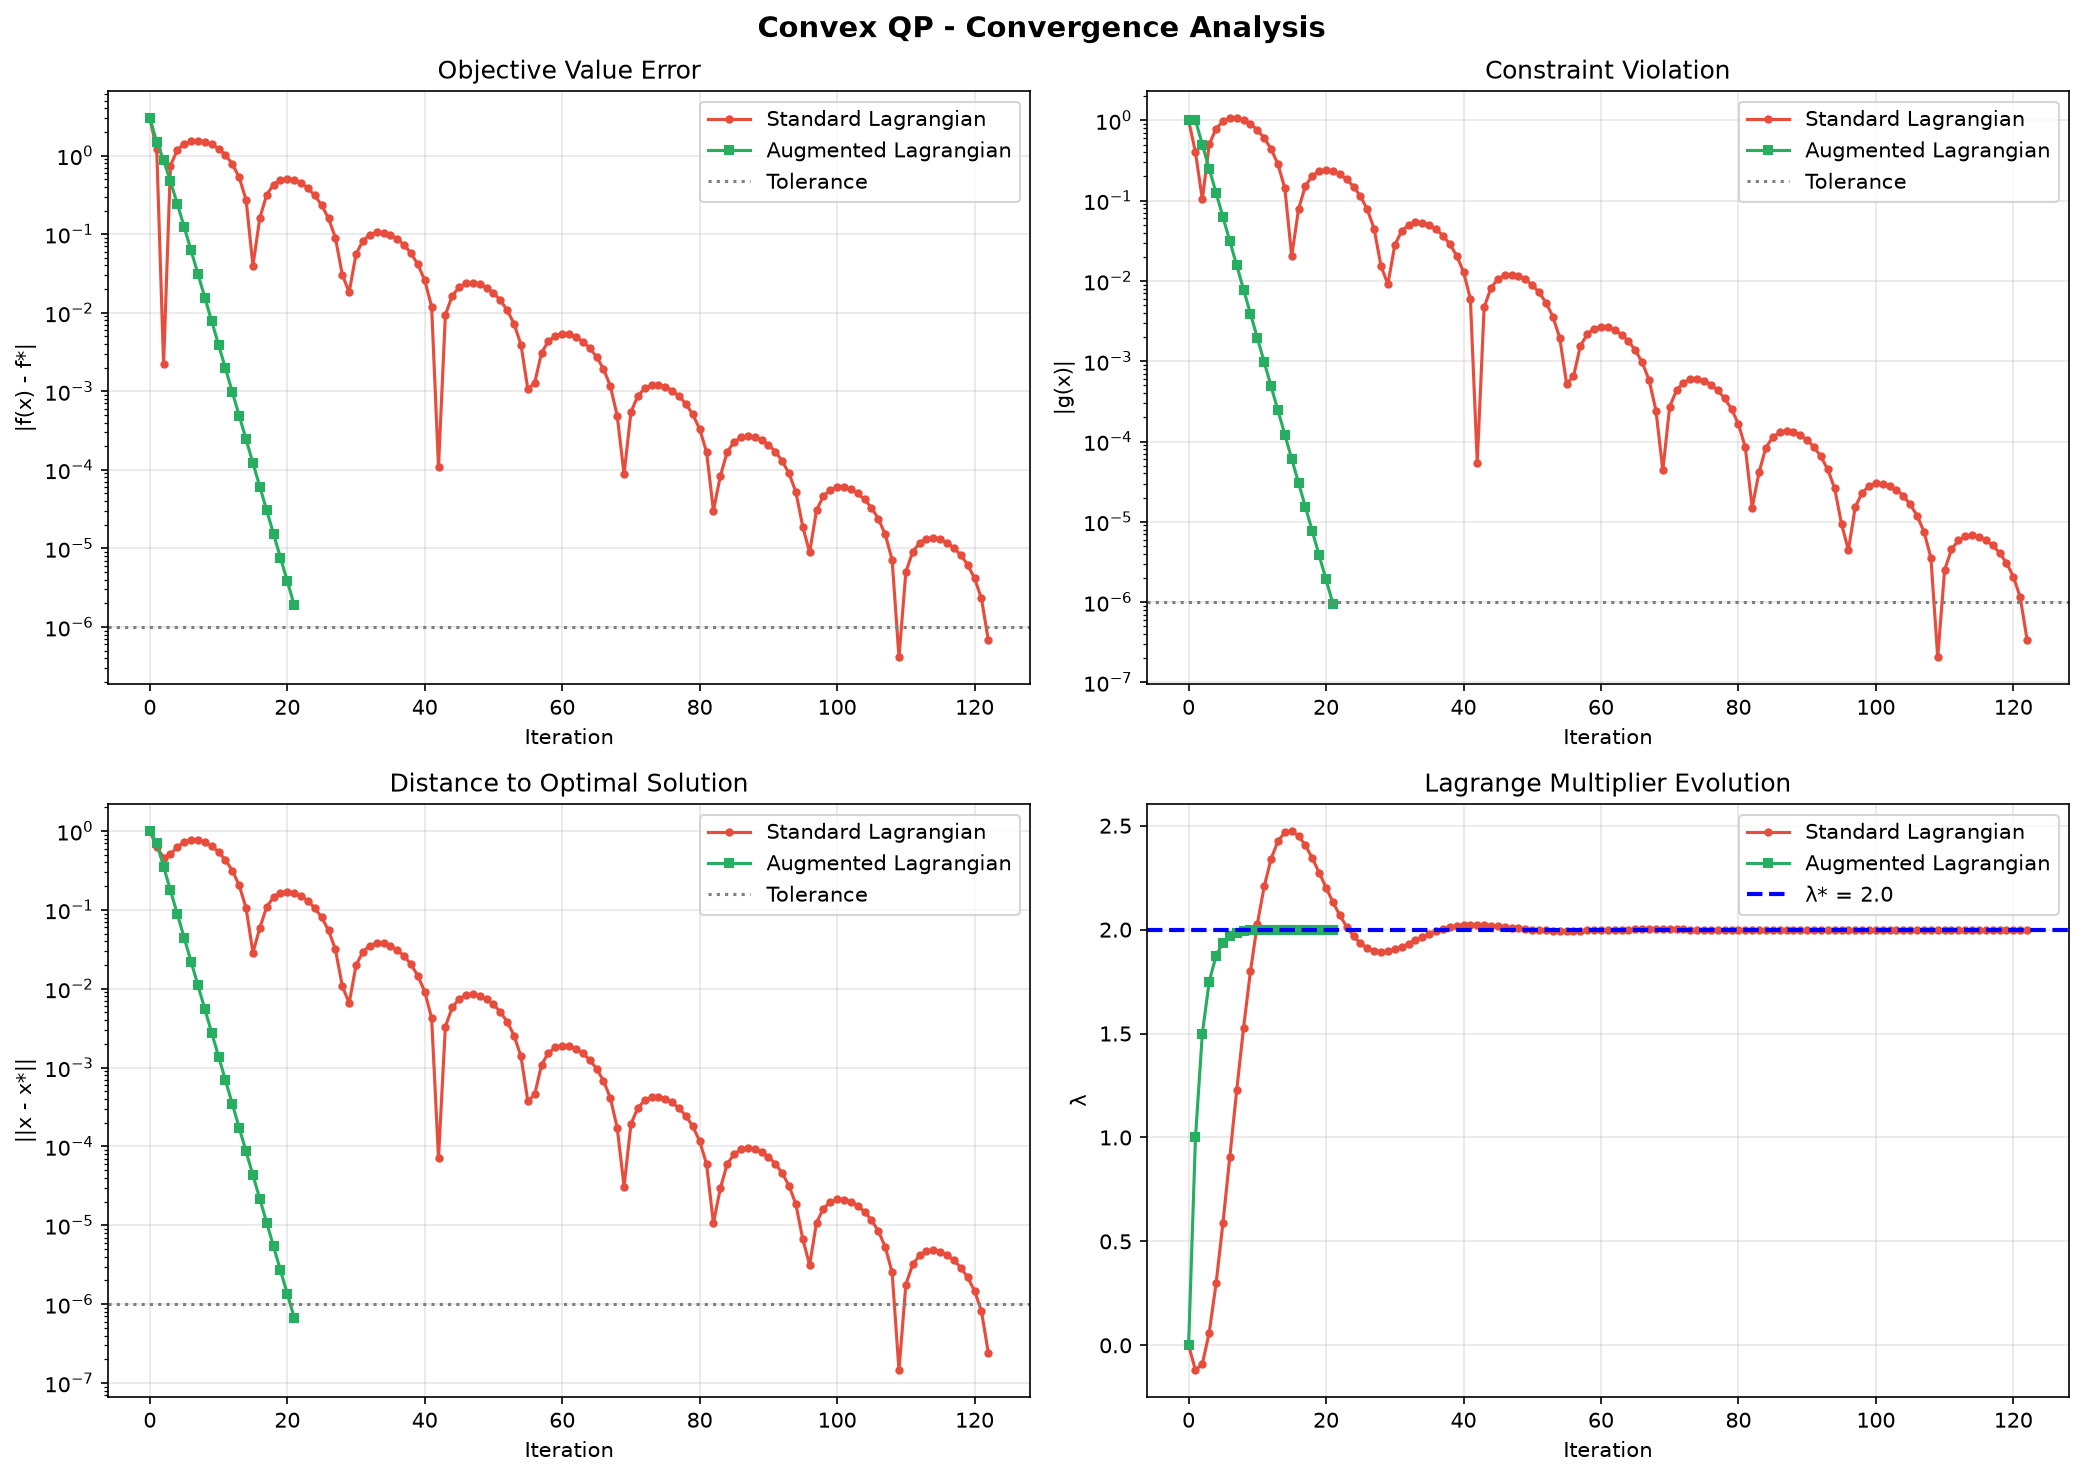
\includegraphics[width=0.75\linewidth]{results/lagrangian_comparison/case_a_convex/02_convergence.png}
  \caption{Case A: convergence history.}
  \label{fig:case-a-convergence}
\end{figure}

\Cref{tab:case-a-summary} reports the terminal objective value and constraint violation.

\begin{table}[H]
  \centering
  \caption{Case A: terminal statistics.}
  \label{tab:case-a-summary}
  \begin{tabular}{@{}l S[table-format=3.0] S[table-format=1.7] S[table-format=1.2e-2]@{}}
    \toprule
    {Method} & {Iters} & {$f(\bm{x}_{\mathrm{final}})$} & {$|c(\bm{x}_{\mathrm{final}})|$} \\
    \midrule
    Standard Lagrangian (dual ascent) & 122 & 1.9999993 & 3.40e-07 \\
    Augmented Lagrangian & 21 & 1.9999981 & 9.52e-07 \\
    \bottomrule
  \end{tabular}
\end{table}

\subsubsection{Case B: nonconvex double-well objective}\label{subsubsec:case-b}
We consider the equality-constrained nonconvex problem
\begin{equation}
  \label{eq:case-b}
  \begin{aligned}
    \min_{(x_1,x_2)\in\R^2}\quad & (x_1^2-1)^2 + x_2^2,\\
    \text{s.t.}\quad & x_1 = 0.
  \end{aligned}
\end{equation}
The constrained optimum is $\bm{x}^\star=(0,0)$ with $f^\star=1$.
The objective has two attractive wells near $x_1=\pm 1$, while the constraint forces $x_1=0$. In our run, the dual-ascent method does not converge within 500 iterations and stalls at $|x_1|\approx 0.22$, whereas the augmented Lagrangian converges in 19 outer iterations to $|x_1|\approx 7\times 10^{-8}$. \Cref{fig:case-b-comparison} compares the resulting trajectories: the dual-ascent iterates are repeatedly attracted to the unconstrained wells and traverse long arcs before returning toward the constraint, while the augmented method moves quickly to the constraint manifold and then contracts toward the constrained minimizer.

\begin{figure}[H]
  \centering
  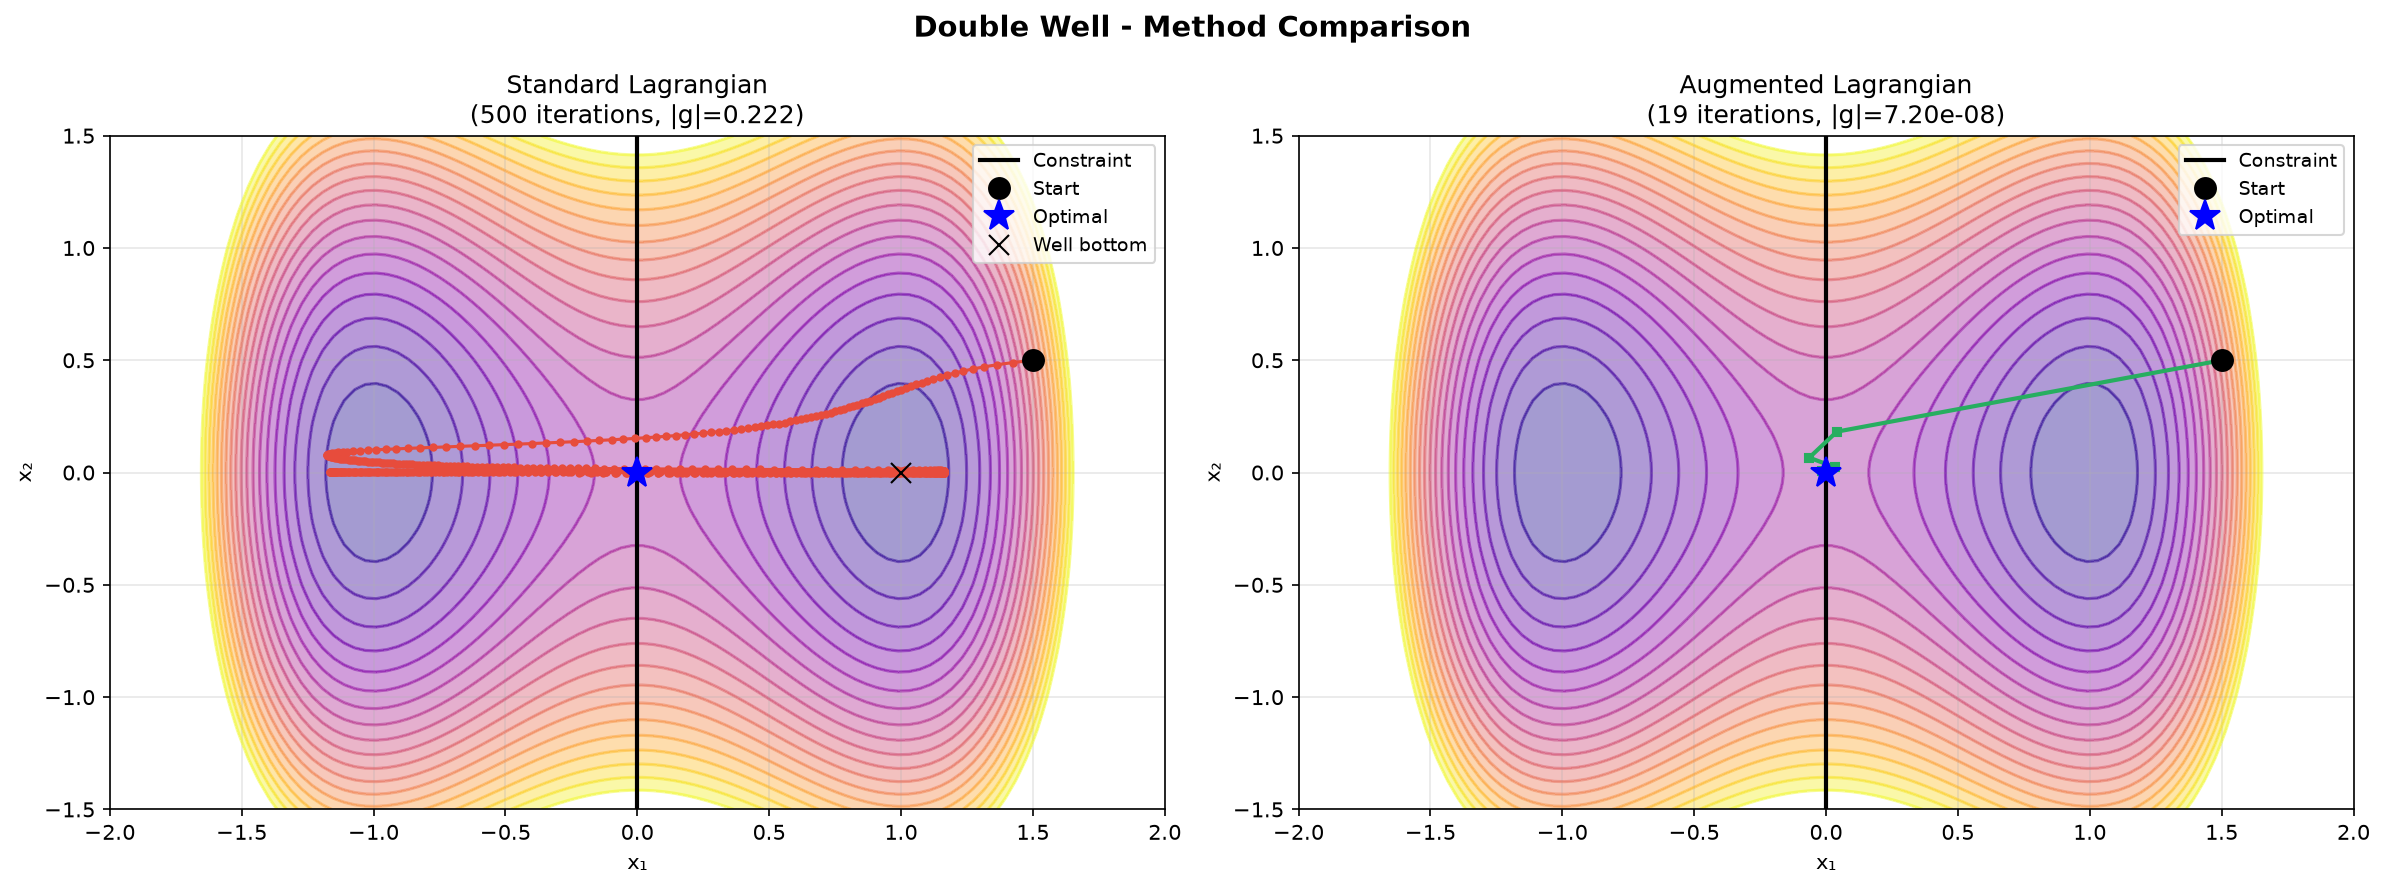
\includegraphics[width=0.98\linewidth]{results/lagrangian_comparison/case_b_nonconvex/08_comparison.png}
  \caption{Case B: trajectories (dual ascent vs.\ AL).}
  \label{fig:case-b-comparison}
\end{figure}

\Cref{tab:case-b-summary} reports the terminal values. Notably, the dual-ascent method attains $f(\bm{x}_{\mathrm{final}})<f^\star$ by settling in an infeasible well, illustrating that objective reduction alone is not a reliable indicator of progress in constrained nonconvex problems.

\begin{table}[H]
  \centering
  \caption{Case B: terminal statistics.}
  \label{tab:case-b-summary}
  \begin{tabular}{@{}l l S[table-format=3.0] S[table-format=1.6] S[table-format=1.2e-2]@{}}
    \toprule
    {Method} & {Converged} & {Iters} & {$f(\bm{x}_{\mathrm{final}})$} & {$|c(\bm{x}_{\mathrm{final}})|$} \\
    \midrule
    Standard Lagrangian (dual ascent) & No & 500 & 0.9040 & 2.22e-01 \\
    Augmented Lagrangian & Yes & 19 & 1.0000 & 7.20e-08 \\
    \bottomrule
  \end{tabular}
\end{table}

The failure mode of the standard Lagrangian in Case B can be understood by examining the merit functions along the slice $x_2=0$. Along this line, the constrained optimum corresponds to $x_1=0$, while the original objective has minima at $x_1=\pm 1$. For a fixed multiplier $\lambda$, the standard Lagrangian
\begin{equation}
  \mathcal{L}(x_1,0;\lambda) = (x_1^2-1)^2 + \lambda x_1
\end{equation}
tilts the two wells but does not eliminate infeasible local minimizers. By contrast, the augmented Lagrangian adds a quadratic term,
\begin{equation}
  \mathcal{L}_\rho(x_1,0;\lambda) = (x_1^2-1)^2 + \lambda x_1 + \frac{\rho}{2}x_1^2,
\end{equation}
which raises the wells and can create a single basin around $x_1=0$ for sufficiently large $\rho$. This landscape shaping is visualized in \cref{fig:case-b-slice} and helps the inner minimization favor feasibility rather than repeatedly returning to the wells.

\begin{figure}[H]
  \centering
  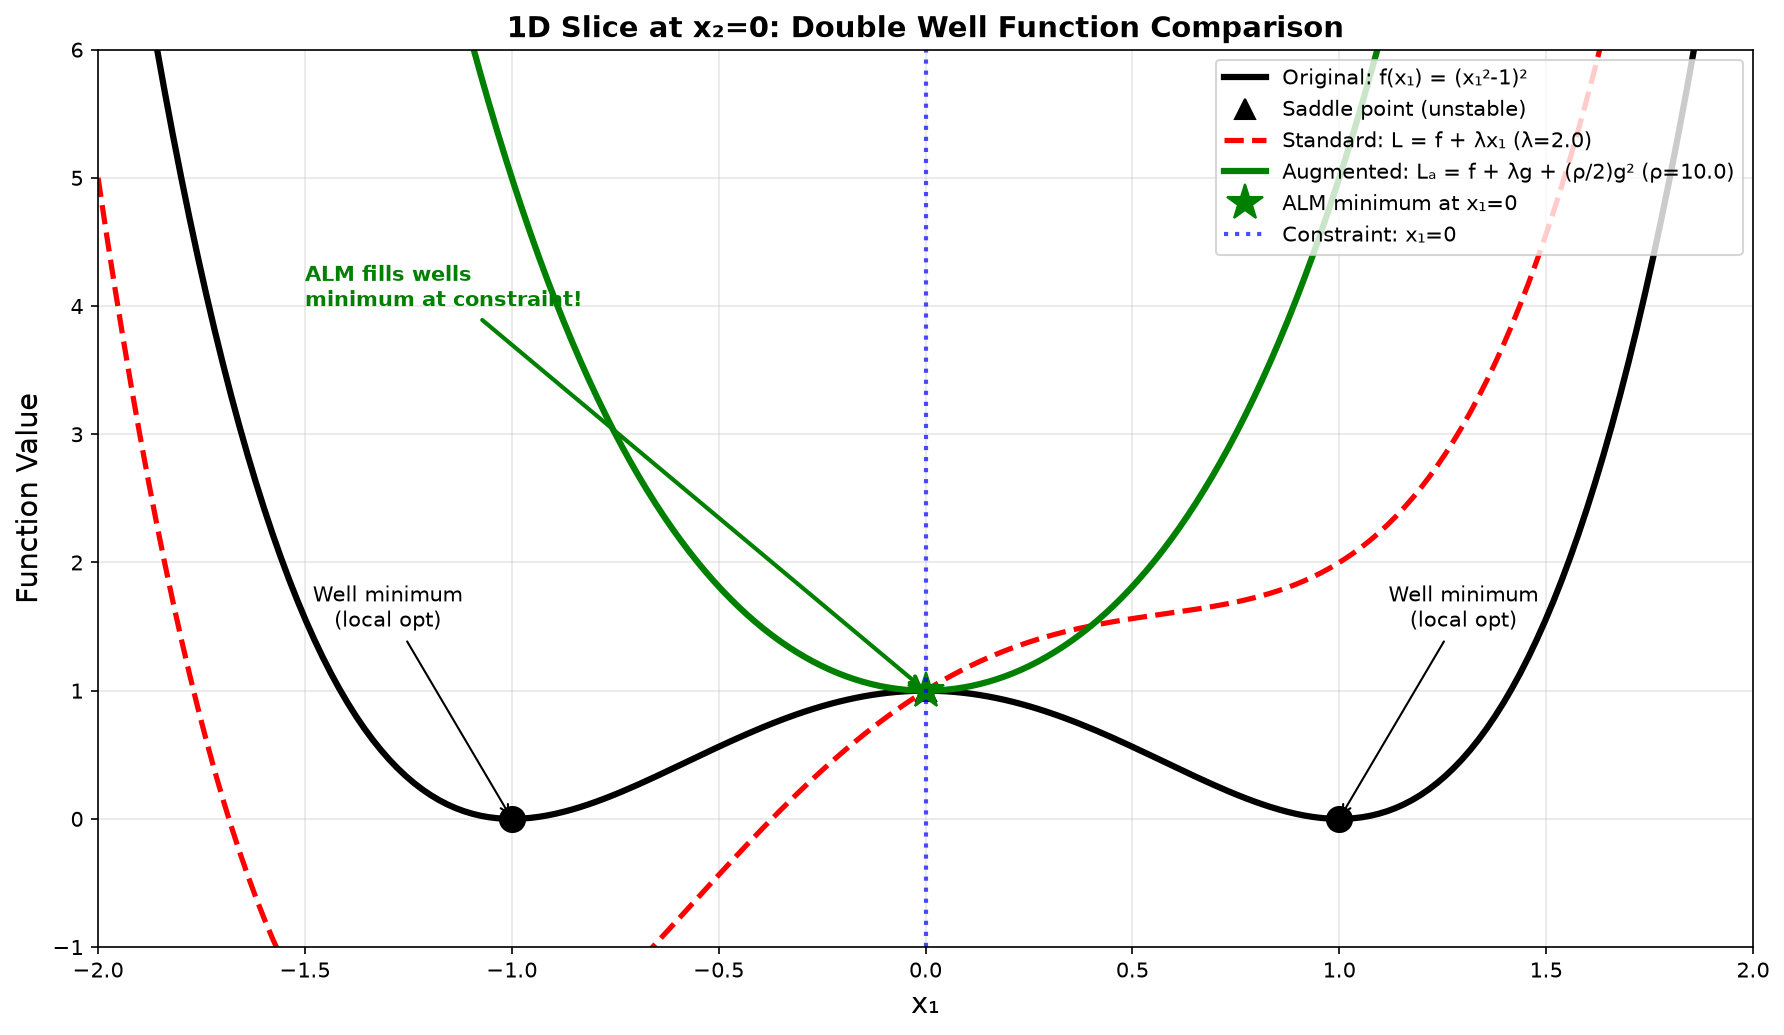
\includegraphics[width=0.95\linewidth]{results/lagrangian_comparison/case_b_nonconvex/06_1d_slice.png}
  \caption{Case B: 1D slice at $x_2=0$.}
  \label{fig:case-b-slice}
\end{figure}

Overall, augmented Lagrangian methods provide a principled way to balance objective reduction and feasibility without extreme penalty growth: multiplier adaptation reduces the need for $\rho\to\infty$ and mitigates ill-conditioning, while the quadratic augmentation can reshape the local landscape near the constraint manifold.\cite{NocedalWright,DufosseHansen} This balance is particularly appealing in black-box optimization, where the unconstrained subproblems are typically solved only approximately under limited evaluation budgets.
The next section (\cref{sec:al-cma-es}) specializes these ideas to the algorithmic setting considered in this project.

\subsection{Adaptive Updates \& Search Guidance}

A static penalty method optimizes
$f(x)+\rho\sum_i \max(0,g_i(x))^2$ with a fixed $\rho>0$.
In comparison-based evolutionary search, this approach is brittle:
if $\rho$ is too small, infeasible points may dominate the ranking and the mean drifts outside;
if $\rho$ is too large, the induced landscape becomes sharply curved near the boundary,
reducing the probability of producing successful steps and triggering premature step-size decrease.
The adaptive AL mechanism addresses this trade-off by separately adapting
(i) multipliers $\lambda$, which set the directional pressure toward feasibility,
and (ii) penalties $\omega$, which control the curvature and conditioning of the penalized landscape.

Adapting the multipliers is crucial because $\lambda$ provides a first-order steering term in the ranking function.
In the active branch of $h(x, \lambda, \omega)$, the constraint contribution $\lambda_i g_i(x)$ induces a selection gradient aligned with $\nabla g_i$ when $g_i(x)>0$.
At a constrained optimum $x_{\mathrm{opt}}$, there exists $\lambda_{\mathrm{opt}}\ge 0$ such that
\[
\nabla f(x_{\mathrm{opt}})
+\lambda_{\mathrm{opt}}\,\nabla g(x_{\mathrm{opt}})=0,
\]
and the augmented Lagrangian satisfies
\begin{equation}
\nabla_x h(x_{\mathrm{opt}},\lambda_{\mathrm{opt}},\omega)
=
\nabla f(x_{\mathrm{opt}})
+\max\!\bigl(0,\lambda_{\mathrm{opt}}+\omega g(x_{\mathrm{opt}})\bigr)\nabla g(x_{\mathrm{opt}})
=0,
\quad \forall\,\omega>0.
\end{equation}
This identity highlights the advantage over pure penalty methods:
once $\lambda_t$ approaches $\lambda_{\mathrm{opt}}$, feasibility can be enforced
without requiring $\omega\to\infty$.

\begin{table}[H]
  \centering
  \caption{Static penalty vs.\ augmented Lagrangian.}
  \label{tab:comparison}
  \begin{tabularx}{\linewidth}{@{} l X X @{}}
    \toprule
    {Feature} & {Static penalty} & {Augmented Lagrangian} \\
    \midrule
    Mechanism &
    Optimize a penalized objective \(f(\bm{x})+\rho\,\norm{\pos{g(\bm{x})}}_2^2\) with fixed \(\rho\). &
    Rank candidates by \(h(\bm{x},\bm{\gamma},\bm{\omega})\) and adapt \((\bm{\gamma},\bm{\omega})\) online. \\
    \addlinespace
    Advantages &
    Minimal state and simple implementation. &
    Enforces feasibility without requiring \(\omega\to\infty\) and reduces tuning sensitivity. \\
    \addlinespace
    Limitations &
    Highly sensitive to \(\rho\): too small yields infeasible optima, too large yields stiff landscapes. &
    Additional state variables and update logic for multipliers and penalties. \\
    \addlinespace
    Effect on step-size &
    Large \(\rho\) can induce step-size collapse near the boundary. &
    Penalties are increased only when needed, helping preserve stable covariance adaptation. \\
    \bottomrule
  \end{tabularx}
\end{table}

\section{AL-CMA-ES Algorithm}\label{sec:al-cma-es}

In this section, we adopt the notation used in the AL-CMA-ES literature~\cite{ArnoldPorter2015,Atamna2016}: the Lagrange multiplier is denoted by $\gamma$ (corresponding to $\lambda$ in \cref{sec:al}) and the penalty coefficient by $\omega$ (corresponding to $\rho$ in \cref{sec:al}). 

\subsection{Integration of the Augmented Lagrangian}

In the standard implementation of CMA-ES, the offsprings sampled are ranked based on their function value. AL-CMA-ES replaces it by ranking them based on the Augmented Lagrangian value:
\begin{equation}
\label{eq:al-cmaes-merit}
h(x, \gamma, \omega) = f(x) + \sum^m_{i=1} \varphi(g_i(x), \gamma^i, \omega^i)
\end{equation}
where 
$$
\varphi(g_i(x), \gamma^i, \omega^i) =
\begin{cases}
    \gamma^i g_i(x) + \frac{\omega^i}{2}g_i(x) ^2 \quad \text{ if } \gamma^i + \omega^i g_i(x) \ge 0 \\
    -\frac{\gamma^{i2}}{2 \omega^i} \qquad \qquad \quad \qquad\text{otherwise}
\end{cases}
$$

Now, a candidate is ranked based on a score depending on both the value of $f$ and the constraint $g$.

\paragraph{Update of the mean, step size and covariance matrix} 
We then update the mean based on the ranking obtained with the usual weighted average, and the step size and covariance matrix with the standard CMA updates.


\paragraph{Update of the Lagrange multiplier} To update $\gamma$, we use a gradient ascent step:
\begin{equation}
\label{eq:al-cmaes-gamma}
\gamma^i_{t+1} = \max (0, \gamma_t^i + \frac{\omega_t^i}{d_\gamma} g_i (m_{t+1}))
\end{equation}
We derive it using the dual problem in which we want to maximize the dual function $D(\gamma) = \min_x \mathcal{L}(x, \gamma)$, with $g(x)$ the gradient with respect to $\gamma$. We thus have the gradient step $\gamma_{t+1} = \gamma_{t} + \alpha g(x)$ with $\alpha$ the step size given by the penalty parameter $\omega$ and a damping factor. 

We can interpret the update as increasing $\gamma$ if $m_{t+1}$ is outside of the feasible space (and thus $g> 0$), this will increase $\gamma g$ and push the next means to feasible solutions. Otherwise, if $m_{t+1}$ is feasible, we decrease $\gamma$ to reduce the "noise" added to the function value in $h$ and allow the next means to possibly approach the boundaries again.

\paragraph{Update of the penalty term} Then, $\omega$ is updated as following:
\begin{equation}
\label{eq:al-cmaes-omega}
\omega^i_{t+1} = 
\begin{cases}
    \omega_t^i . \chi^{1/(4d_\omega)} \quad \text{if Condition 1 or Condition 2 is met}\\
    \omega_t^i . \chi^{-1/d_\omega} \quad \text{ otherwise}
\end{cases}
\end{equation}
where $\chi = 2^{1/n}$ and $d_\omega$ are some given constants.

To understand this update, we need to study the conditions determining when to increase $\omega$. These conditions where derived by Arnold \& Porter in \cite{ArnoldPorter2015} analyzing a step of the $(1+1)$-ES on a linear constraint problem.

\paragraph{Condition 1}
$$
\omega_t g(m_{t+1})^2 <
k_1\,\dfrac{|h(m_{t+1},\gamma_t,\omega_t)-h(m_t,\gamma_t,\omega_t)|}{n}
$$
This condition relies on the fact that the function~\eqref{eq:al-cmaes-merit} changes from iteration $t$ to $t+1$ due to change in the primal space, $\Delta h_x \approx |h(m_{t+1}) - h(m_t)|$ (the change in $h$ keeping $\gamma$ and $\omega$ constant). And change in the dual space, $\Delta h_{\gamma, \omega} \approx \omega g ^2$, because $\Delta \gamma \approx \omega g(y)$.

The condition becomes $\Delta h_{\gamma, \omega} < \frac{k_1}{n} \Delta h_x$, it means that we increase $\omega$ if the change in $h$ induced by the constraint term update is significantly smaller than the change induced by the optimization of $f$. 
It's triggered when the correction from the Lagrange multiplier update is too "weak" to influence how the mean will move at the next step, when the dual update is too slow compared to the primal update.
Since $\omega$ acts as step size for $\gamma$, increasing it will increase the magnitude of its update and balance the magnitude of the primal update. 
The normalization by $n$ ensures that the condition is scale invariant to the problem dimension.

\begin{figure}[H]
    \centering
    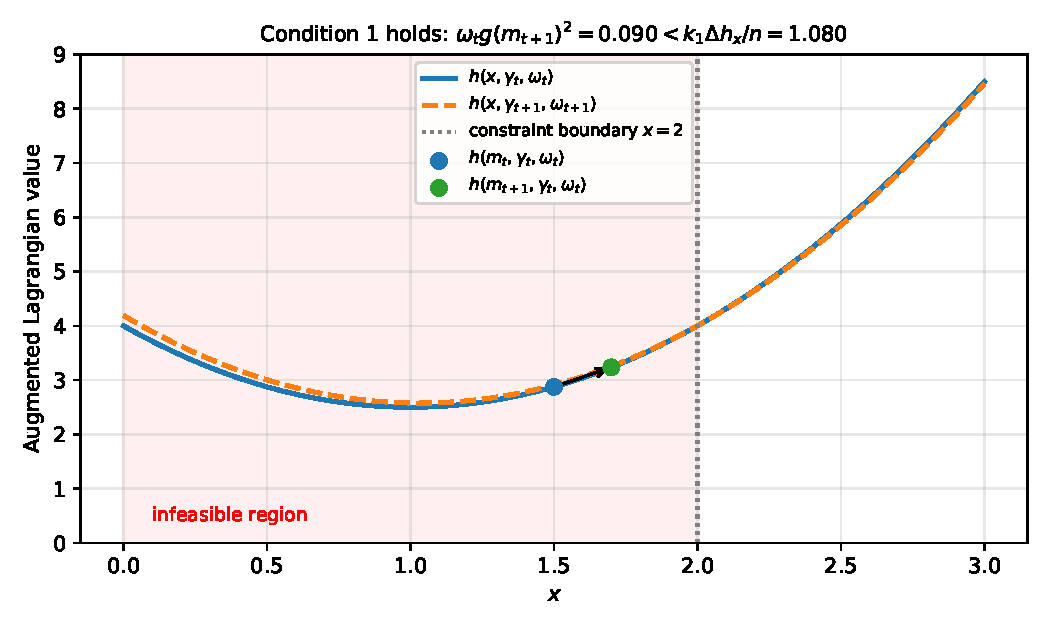
\includegraphics[width=0.7\textwidth]{results/report_figures/condition1.pdf}
    \caption{Trigger of Condition 1 on $f(x) = x^2$, with $g(x) = 2 - x$.}
    \label{fig:condition1}
\end{figure}

\paragraph{Condition 2}
$$
k_2\,|g_i(m_{t+1})-g_i(m_t)|<|g_i(m_{t+1})|
$$
This condition is used to avoid stagnation, if we are in a non feasible space, we want the $g_i$ term to decrease geometrically to $0$. If the inequality holds, the absolute value of the constraint decreases too slowly compared to its magnitude. This happens usually when the gradient of $f$ (pointing to the infeasible region since the constraint is active at $x_{\text{opt}}$) balances the gradient of the Lagrangian term (pointing to the feasible region). Increasing $\omega$ increases the strength of the gradient pointing to the feasible set, breaking this balance. 

\begin{figure}[H]
    \centering
    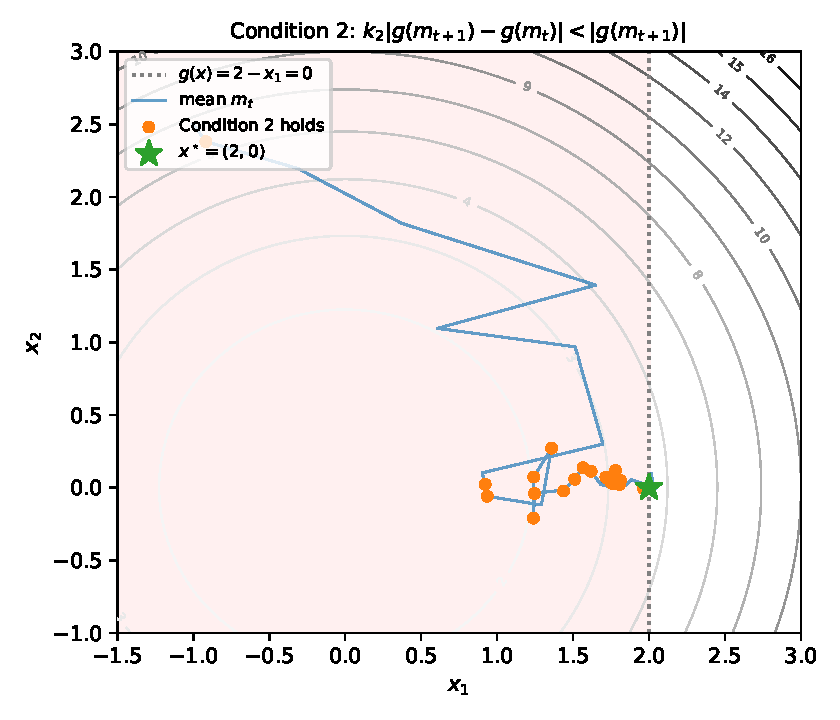
\includegraphics[width=0.5\textwidth]{results/report_figures/condition2.pdf}
    \caption{Trigger of Condition 2 on $f(x) = \sum^2_{i=1}x_i^2$, with $g(x) = 2 - x_1$.}
    \label{fig:condition2}
\end{figure}

\paragraph{AL-CMA-ES} The final algorithm is the following:
\begin{algorithm}[H]
\caption{$(\mu/\mu_w, \lambda)$-ES with Augmented Lagrangian Constraint Handling}
\begin{algorithmic}[1]
\State \textbf{Initialize} mean $m_0 \in \mathbb{R}^n$, step size $\sigma_0$, covariance $C_0=\mathbf{I}$, multipliers $\gamma_0$, penalties $\omega_0$.
\State Set weights $w_1,\dots,w_\mu$.
\While{stopping criterion not met}
    \State \textbf{Sample} $\lambda$ offspring: $x_k = m_t + \sigma_t y_k$, with $y_k \sim \mathcal{N}(0, C_t)$ for $k=1,\dots,\lambda$.
    \State \textbf{Selection}: sort $x_{1:\lambda},\dots,x_{\lambda:\lambda}$ by $h(x_k,\gamma_t,\omega_t)$.
    \State \textbf{Update mean:} $m_{t+1} = m_t + \sigma_t \sum_{i=1}^{\mu} w_i\, y_{i:\lambda}$.
    \State \textbf{Update CMA parameters:} update $\sigma_{t+1}$ and $C_{t+1}$ (standard CMA-ES rules).
    \State \textbf{Update multipliers $\forall i \in \{1,...,m\}$:}
          $\gamma_{t+1}^i = \max\!\left(0,\, \gamma_t^i + \frac{\omega_t^i}{d_\gamma} g_i(m_{t+1})\right)$.
    \State \textbf{Update penalties $\forall i \in \{1,...,m\}$:}
    \If{Condition 1 or Condition 2 holds}
        \State $\omega_{t+1}^i = \omega_t^i \chi^{1/(4d_\omega)}$.
    \Else
        \State $\omega_{t+1}^i = \omega_t^i \chi^{-1/d_\omega}$.
    \EndIf
    \State $t \leftarrow t+1$.
\EndWhile
\end{algorithmic}
\end{algorithm}

\subsection{Surrogate-assisted augmented Lagrangian variant}\label{subsec:surrogate-al}
The update rules above implicitly rely on constraints that are sufficiently smooth at the boundary so that multiplier adaptation can approximate KKT conditions. For non-smooth constraints, Dufoss\'e and Hansen\cite{DufosseHansen} show that the estimated multiplier can oscillate between values associated with different one-sided derivatives, and the penalty coefficient can increase unnecessarily when the constraint becomes uninformative in the feasible region. To mitigate these effects, they propose replacing the original constraint by a local surrogate model when evaluating the AL merit function and updating the AL state.

For a constraint $g_k$, the surrogate is constructed from recently observed infeasible points. Let $D_k^{(t)}$ denote a set of the most recent $\kappa$ points with $g_k(\bm{x})>0$ together with their constraint values. Choose a reference point $\bm{c}_k^{(t)}$ near the active boundary. In the typical case where the constraint can be evaluated on both sides, $\bm{c}_k^{(t)}$ is taken as the current mean $m^{(t)}$; when $g_k$ is constant in the feasible region, $\bm{c}_k^{(t)}$ is instead obtained by a short line search between $m^{(t)}$ and the nearest infeasible point.\cite{DufosseHansen} A linear regression without intercept is then fitted on centered data,
\begin{equation}
  \label{eq:surrogate-fit}
  \hat{\theta}
  =
  \argmin_{\theta\in\R^n}
  \sum_{\bm{x}\in D_k^{(t)}}
  \bigl(\theta^\top(\bm{x}-\bm{c}_k^{(t)}) - (g_k(\bm{x})-g_k(\bm{c}_k^{(t)}))\bigr)^2,
\end{equation}
leading to the local surrogate
\begin{equation}
  \label{eq:surrogate-def}
  \hat{g}_k^{(t)}(\bm{x})
  =
  \hat{\theta}^\top(\bm{x}-\bm{c}_k^{(t)}) + g_k(\bm{c}_k^{(t)}).
\end{equation}
By construction, $\hat{g}_k^{(t)}(\bm{c}_k^{(t)})=g_k(\bm{c}_k^{(t)})$, and the model smooths the constraint signal used by the AL updates near the boundary. In the surrogate-assisted variant, the AL merit function in~\eqref{eq:al-cmaes-merit} and the update rules in~\eqref{eq:al-cmaes-gamma}--\eqref{eq:al-cmaes-omega} are evaluated with $\hat{g}_k^{(t)}$ instead of $g_k$.\cite{DufosseHansen} Constraint evaluations are still performed to update the surrogate model and to report feasibility, but selection pressure is driven by the smoothed constraint signal, which avoids introducing the surrogate-assisted variant abruptly when discussing the non-smooth benchmark in \cref{subsubsec:exp-nonsmooth}.

\subsection{Convergence Properties}

\cite{Atamna2017} analyze the convergence of an augmented-Lagrangian evolution strategy
under multiple active linear inequality constraints using a Markov-chain framework.
They adopt the notion of almost sure linear convergence:
a sequence $(X_t)$ converges linearly to $x_{\mathrm{opt}}$ if there exists $CR>0$ such that
\begin{equation}
\lim_{t\to\infty}\frac{1}{t}
\ln\frac{\|X_t-x_{\mathrm{opt}}\|}{\|X_0-x_{\mathrm{opt}}\|}
=-CR,
\quad \text{a.s.}
\tag{2.6}
\end{equation}

Their theoretical setting assumes:
(i) a unique global optimum $x_{\mathrm{opt}}$;
(ii) all constraints active at $x_{\mathrm{opt}}$;
(iii) differentiability of $f$ and the constraints at $x_{\mathrm{opt}}$;
and (iv) the linear independence constraint qualification (LICQ),
which yields a unique multiplier vector $\lambda_{\mathrm{opt}}$.
Under these assumptions, sufficient conditions are provided for almost sure linear convergence of
the iterates $X_t\to x_{\mathrm{opt}}$,
the multiplier estimates $\lambda_t\to \lambda_{\mathrm{opt}}$,
and the step-size $\sigma_t\to 0$,
expressed in terms of positive Harris recurrence and integrability properties
of the associated homogeneous Markov chain.

Complementing this theory,
\cite{Atamna2016} report empirical linear convergence of a
$(\mu/\mu_w,\lambda)$-MSR-CMA-ES variant with augmented Lagrangian handling
on linearly constrained convex quadratics and ill-conditioned test functions,
emphasizing the importance of covariance adaptation.
Finally, \cite{ArnoldPorter2015} provide a mechanistic stability condition:
the penalty parameter $\omega$ must remain in a regime that avoids excessive ill-conditioning
while still being large enough to prevent stagnation;
their multiplicative update is designed to keep $\omega$ away from extreme values
by reacting to observable progress ratios in $h$ and $g$.


\section{Numerical Experiments \& Discussion}

\subsection{Experimental Setup}\label{subsec:exp-setup}
Our numerical experiments aim to isolate how constraint handling affects CMA-ES dynamics,
with a particular focus on (i) convergence to the constrained optimum, (ii) step-size and
covariance adaptation, and (iii) robustness to ill-conditioning and non-smooth constraints.
We report two complementary views:
(1) the intrinsic convergence behavior of AL-CMA-ES on a smooth linearly constrained quadratic,
and (2) a broader comparison across three benchmark scenarios capturing feasibility enforcement,
scaling, and non-smoothness effects.

\paragraph{Algorithms compared.}
Depending on the scenario, we compare AL-CMA-ES with several baselines commonly used in
constrained black-box optimization:
\emph{Vanilla (no CH)} (ignoring constraints), \emph{Death Penalty},
\emph{Static Quadratic Penalty} (with fixed coefficient $\beta$),
\emph{Adaptive Penalty}, and (for the non-smooth case) a \emph{Surrogate-assisted AL} variant.
All methods are run with identical CMA-ES core settings within each scenario
(same initialization, population parameters, and termination rules), differing only in how
constraints are handled and how candidates are ranked/selected.

\paragraph{Performance indicators.}
We track (i) the distance to the constrained optimum $\|m_t-\bm{x}^\star\|$,
(ii) step-size evolution $\sigma_t$, (iii) constraint violation $g(\bm{x})$,
and (when relevant) internal AL states such as the multiplier $\gamma$ and covariance
conditioning. Evaluation budgets are fixed per benchmark, and all convergence curves are
plotted against the number of objective evaluations.

\paragraph{Default hyperparameters.}
To ensure reproducibility, \cref{tab:al-hyperparams} lists the default values of the AL-CMA-ES hyperparameters as implemented in the \texttt{cma} Python package~\cite{Atamna2017,ArnoldPorter2015}. These values are used in all experiments unless otherwise noted.

\begin{table}[H]
  \centering
  \caption{AL-CMA-ES hyperparameters and their default values.}
  \label{tab:al-hyperparams}
  \begin{tabular}{@{}l l p{0.55\linewidth}@{}}
    \toprule
    {Symbol} & {Default Value} & {Description} \\
    \midrule
    $\chi$ & $2^{1/n}$ & Base factor for penalty update \\
    $d_\gamma$ & $5$ & Damping factor for multiplier update \\
    $d_\omega$ & $5$ & Damping exponent for penalty update (via $\chi^{1/(4d_\omega)}$) \\
    $k_1$ & $3$ & Threshold for Condition~1 (primal-dual balance) \\
    $k_2$ & $5$ & Threshold for Condition~2 (stagnation detection) \\
    $\gamma_0$ & $0$ & Initial Lagrange multiplier \\
    $\omega_0$ & $1$ & Initial penalty coefficient \\
    \bottomrule
  \end{tabular}
\end{table}
\subsection{Convergence Behavior of AL-CMA-ES}

We first examine the intrinsic convergence behavior of AL-CMA-ES,
focusing on the evolution of the distance to the constrained optimum,
the internal step-size dynamics, and the robustness of the adaptation phase.

% --- Insert Figure: Distance ---
\begin{figure}[htbp]
    \centering
    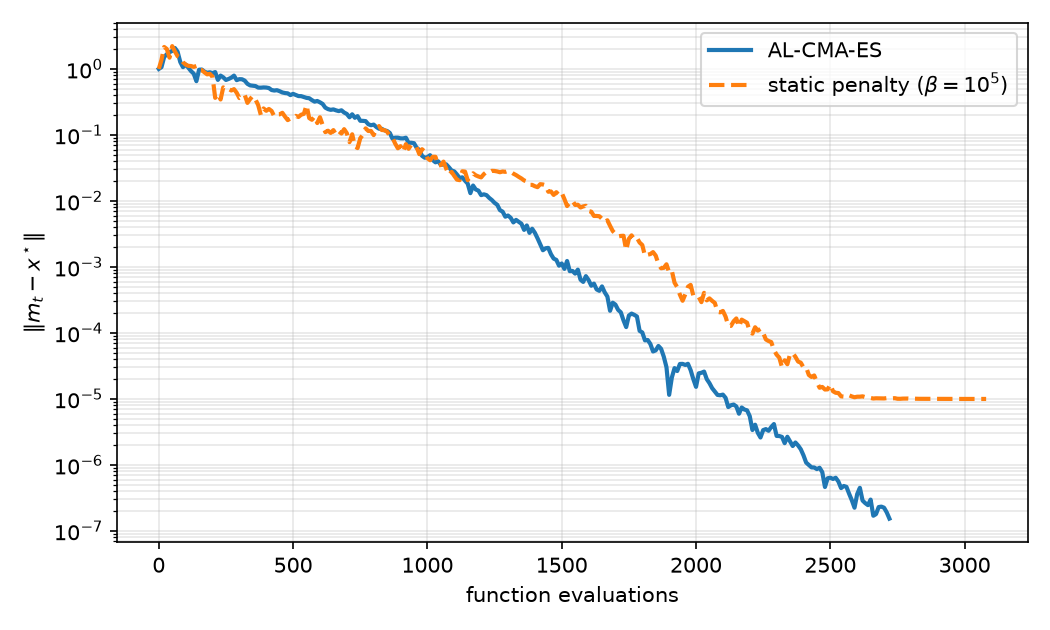
\includegraphics[width=0.7\textwidth]{results/report_figures/al_vs_static_distance.png}
    \caption{Distance to constrained optimum: $\|m_t-x^\star\|$ vs. evaluations (semilog scale).}
    \label{fig:dist}
\end{figure}
% ---------------------------------

\paragraph{Distance to the optimum.}
The distance $\|m_t-x^\star\|$ decreases approximately linearly on a logarithmic scale
for both methods, indicating a near-linear convergence regime
with respect to the iteration count (and equivalently the number of evaluations,
given a fixed population size); see Figure~\ref{fig:dist}.
We run both methods on the sphere $f(\bm{x})=\norm{\bm{x}}_2^2$ in dimension $n=10$ with the linear constraint $x_1\ge 1$ (the benchmark of \cref{subsec:exp-comparison}), from $\bm{x}^{(0)}=\bm{0}$ with $\sigma_0=1$, a single seeded run, and a static quadratic penalty $\beta=10^5$ for the baseline (script \texttt{report\_figures.py}).
Empirically, AL-CMA-ES converges faster and reaches higher precision,
achieving distances on the order of $10^{-7}$,
whereas the static penalty method stagnates around $10^{-5}$.
While both trajectories exhibit overall linear decay,
the AL-CMA-ES curve maintains a more consistent convergence rate,
whereas the static-penalty curve is slightly less steep and more irregular.
This behavior suggests that the fixed trade-off encoded in $F_\rho$
increasingly interferes with fine-scale refinement near the constrained optimum.

\paragraph{Step-size evolution.}
The step-size $\sigma_t$ exhibits an approximately linear decay on a log-scale
for both methods (see Figure~\ref{fig:step}), which is a key indicator of algorithmic stability.
In particular, the augmented Lagrangian mechanism does not destabilize
the internal step-size adaptation of CMA-ES.
Instead, AL-CMA-ES preserves the smooth contraction pattern
typically observed on well-behaved problems.
The static-penalty baseline shows a slightly slower and less regular contraction,
consistent with the mild slow-down observed in the distance curve.

\begin{figure}[H]
    \centering
    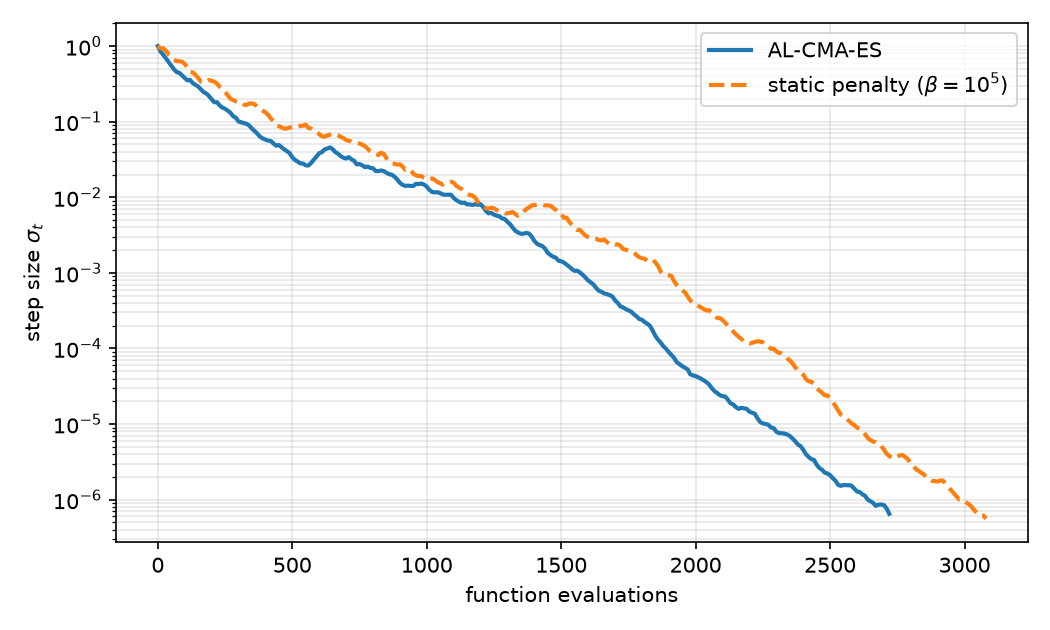
\includegraphics[width=0.7\textwidth]{results/report_figures/al_vs_static_sigma.png}
    \caption{Step-size evolution: $\sigma_t$ vs. evaluations (semilog scale).}
    \label{fig:step}
\end{figure}


\paragraph{Adaptation Phase and Robustness.}
The empirical results observed in \cite{Atamna2017} show that the Augmented Lagrangian is effective on linearly constrained convex quadratic problems, testing it on the Sphere and Ellipsoid functions.
It specifically shows robustness with respect to the number of constraints, \(m \in \{1, 2, 5, 9\}\), and to the initialization of the penalty term, \(\omega \in \{10^{-3}, 1, 10^3\}\), in dimension \(n = 10\).

The algorithm achieves linear convergence to the primal optimum \(x_{\text{opt}}\) and the dual optimum \(\gamma_{\text{opt}}\). This convergence is characterized by an adaptation phase with a duration depending on the choice of \(\omega_0\).
During this phase, \(\omega\) changes until it reaches a stationary distribution depending on the problem dimension and constraints. If we initialize it with a value far from this stationary state, the algorithm spends the initial iterations to adjust \(\omega\) (according to the conditions explained before) until it stabilizes. Once \(\omega\) is stable, the system starts linear convergence to the optimum.

This phase shows that the algorithm is robust to poor initialization. Even when starting with a too small or too large penalty, the Markov chain associated with the algorithm stabilizes, leading to global convergence.


% ============================================================
\subsection{Performance comparisons across three scenarios}\label{subsec:exp-comparison}
This subsection addresses the optional objective of comparing AL-CMA-ES with standard CMA-ES and simple penalty approaches. We consider three scenarios: a single linear constraint on a well-conditioned quadratic objective, an ill-conditioned ellipsoid with an active linear constraint, and a non-smooth constraint with a gradient discontinuity. Together, they highlight how feasibility enforcement, scaling, and non-smoothness affect constrained black-box optimization.

\subsubsection{Linear constraint benchmark}\label{subsubsec:exp-linear}
We first consider a smooth objective with a single linear inequality constraint:
\begin{equation}
\label{eq:baseline-sphere}
  \begin{aligned}
    \min_{\bm{x}\in\R^{10}}\quad & \sum_{i=1}^{10} x_i^2,\\
    \text{s.t.}\quad & 1-x_1 \le 0.
  \end{aligned}
\end{equation}
Defining $g(\bm{x}) := 1-x_1$, the constrained optimum is $\bm{x}^\star=(1,0,\dots,0)$ with $f(\bm{x}^\star)=1$. All methods start from $\bm{x}^{(0)}=\bm{0}$ with $\sigma_0=1$ and run under a budget of 10\,000 objective evaluations.

\textbf{Benchmark structure and optimality conditions.}
This problem has two features that make it a useful diagnostic for constraint handling. First, the unconstrained minimizer $\bm{0}$ is strictly infeasible since $g(\bm{0})=1$. Second, the constrained optimum lies on the active boundary $g(\bm{x}^\star)=0$, so progress requires both reaching feasibility and then contracting along the boundary.

The Karush--Kuhn--Tucker (KKT) conditions also give a convenient reference value for the multiplier. With Lagrangian
\(
  \mathcal{L}(\bm{x},\lambda)= f(\bm{x}) + \lambda(1-x_1),
\)
stationarity at $\bm{x}^\star$ yields
\begin{equation}
  \nabla f(\bm{x}^\star) + \lambda^\star \nabla g(\bm{x}^\star) = 0
  \quad\Longrightarrow\quad
  2\bm{x}^\star - \lambda^\star \bm{e}_1 = \bm{0},
\end{equation}
so $\lambda^\star=2$. This value will be used below to interpret the evolution of the AL multiplier.

\textbf{Convergence and feasibility behavior.}
We compare five strategies: \emph{Vanilla (no CH)} (ignoring $g$), \emph{Death Penalty}, \emph{Static} ($\beta=1$), \emph{Adaptive Penalty}, and \emph{AL-CMA-ES}.\cite{DufosseHansen,Atamna2016} The median convergence curves in \cref{fig:exp-linear-convergence} show that the vanilla baseline rapidly approaches the unconstrained minimizer $\bm{0}$ and then stagnates at distance $\norm{\bm{0}-\bm{x}^\star}_2=1$. The static penalty ($\beta=1$) similarly stagnates at a nonzero distance because the penalty is too weak to enforce feasibility.

This plateau can be explained analytically: restricting to $x_2=\cdots=x_{10}=0$ and $x_1\le 1$, the static penalty objective is
\(
  x_1^2 + \beta(1-x_1)^2,
\)
which is minimized at $x_1=\beta/(1+\beta)$. For $\beta=1$, this gives $x_1=0.5$, hence $g=0.5$ and $f=0.25$, matching the terminal values in \cref{tab:exp-linear-summary}.
\begin{figure}[H]
  \centering
  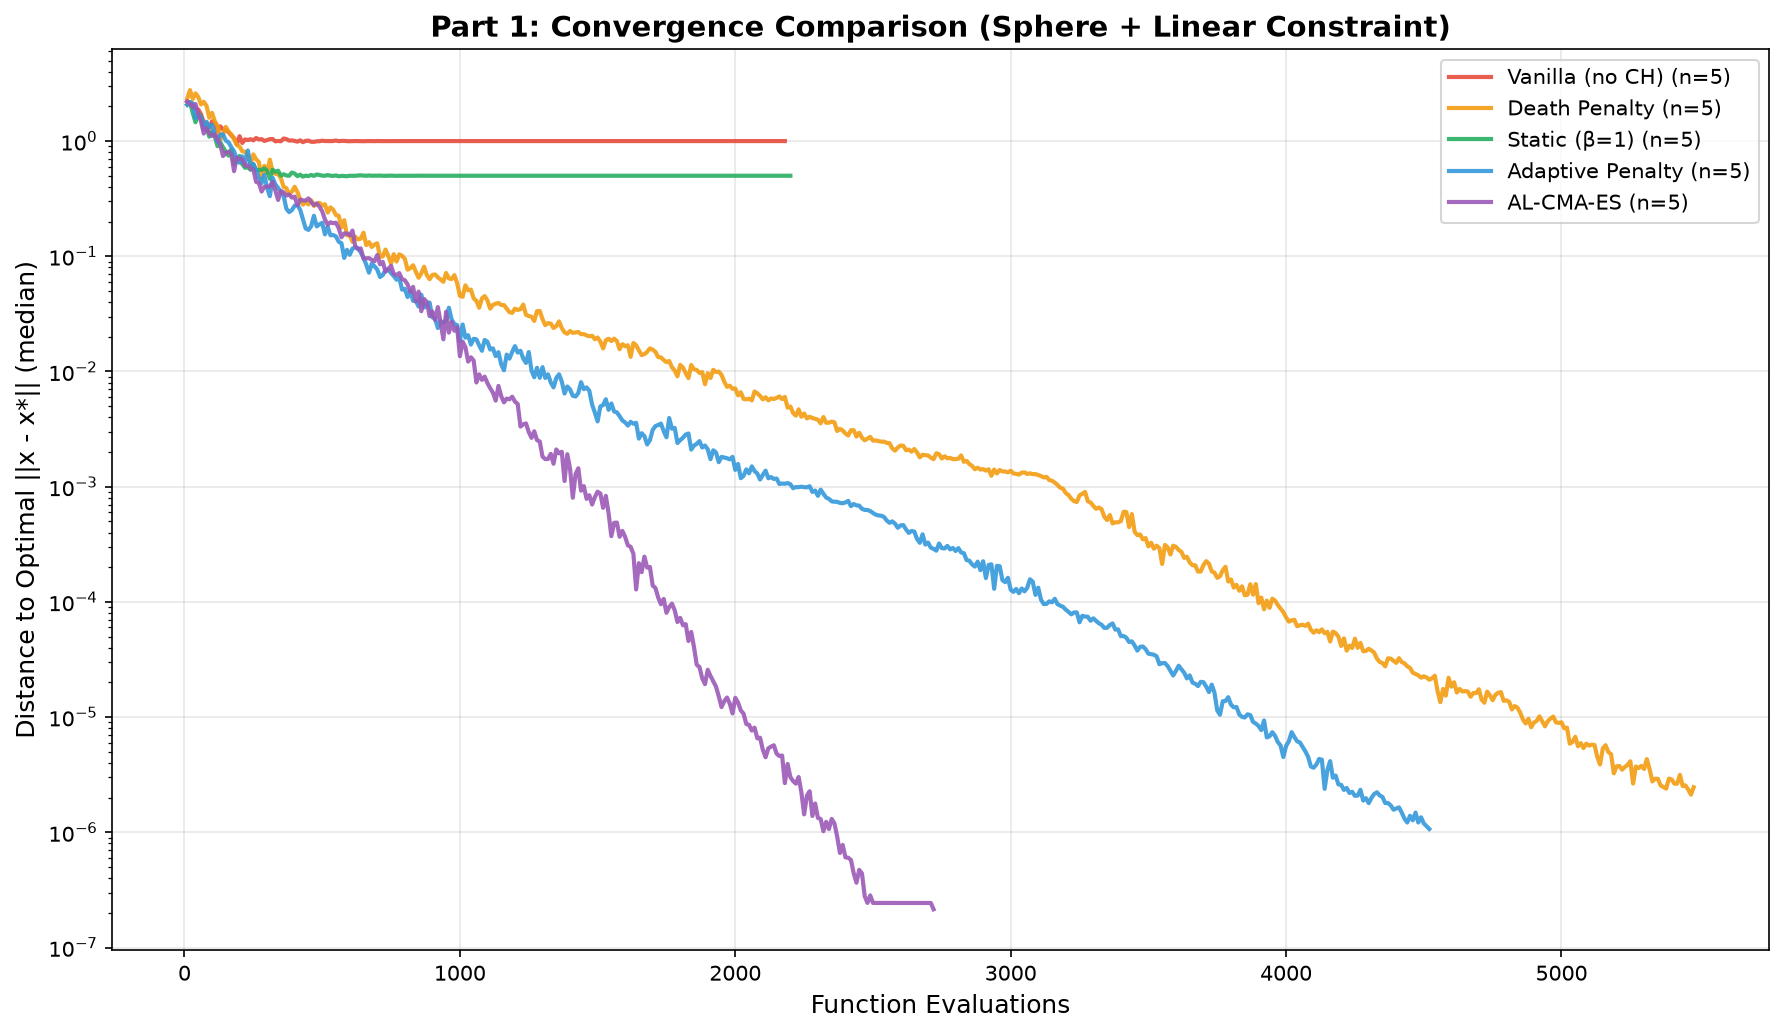
\includegraphics[width=0.92\linewidth]{results/alcmaes_comparison/part1_baseline/01_convergence_median.png}
  \caption{Linear constraint: median convergence.}
  \label{fig:exp-linear-convergence}
\end{figure}

To separate objective progress from feasibility enforcement, \cref{fig:exp-linear-feasibility} reports the constraint value $g(\bm{x})$ over the search.Death penalties enforce feasibility by construction, so $g(\bm{x})$ stays at or below zero after a brief transient, which can also maintain a nonzero slack even though the optimum lies on the active boundary. In contrast, AL-CMA-ES reduces $g(\bm{x})$ progressively and reaches the boundary after an initial phase in which objective improvement and feasibility are balanced; once the violation is close to zero, its distance to $\bm{x}^\star$ contracts rapidly. The adaptive penalty attains feasibility early as its penalty factor grows, but this comes with a strong dependence on the penalty update dynamics.

\begin{figure}[H]
  \centering
  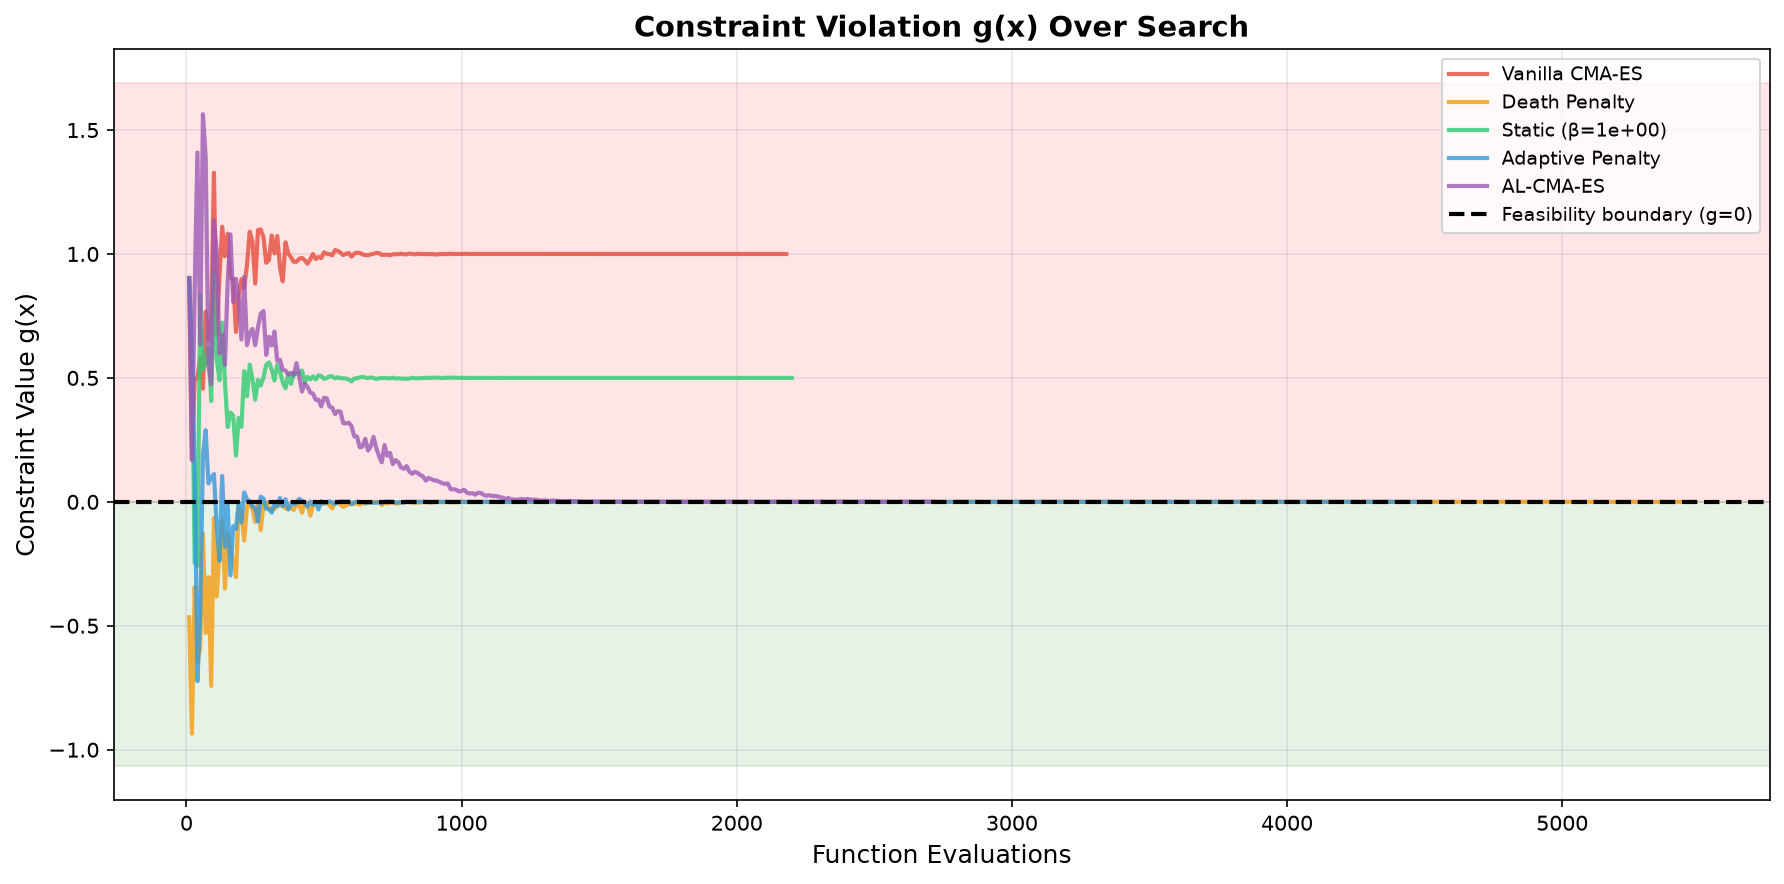
\includegraphics[width=0.92\linewidth]{results/alcmaes_comparison/part1_baseline/06_constraint_violation.png}
  \caption{Linear constraint: constraint violation.}
  \label{fig:exp-linear-feasibility}
\end{figure}


\begin{table}[H]
  \centering
  \caption{Linear constraint: terminal statistics.}
  \label{tab:exp-linear-summary}
  \begin{tabular}{@{}l S[table-format=1.6] S[table-format=1.6] S[table-format=3.0] S[table-format=5.0]@{}}
    \toprule
    {Method} & {$f(\bm{x}_{\mathrm{final}})$} & {$g(\bm{x}_{\mathrm{final}})$} & {Feasible (\%)} & {FEvals} \\
    \midrule
    Vanilla (no CH) & 0.000000 & 1.000000 & 0 & 2110 \\
    Death Penalty & 1.000000 & 0.000000 & 100 & 5860 \\
    Static ($\beta=1$) & 0.250000 & 0.500000 & 0 & 2200 \\
    Adaptive Penalty & 1.000000 & 0.000000 & 100 & 4580 \\
    AL-CMA-ES & 1.000000 & 0.000000 & 100 & 2590 \\
    \bottomrule
  \end{tabular}
\end{table}
Terminal statistics in \cref{tab:exp-linear-summary} summarize this trade-off. While vanilla and static penalties terminate early, they do so at infeasible stationary points of their respective merit functions. Among the feasible methods, AL-CMA-ES reaches the constrained solution with fewer objective evaluations (median 2590) than both the death-penalty baseline (median 5860) and the adaptive penalty scheme (median 4580). This gap is consistent with \cref{fig:exp-linear-feasibility}: death penalties effectively ignore infeasible samples and therefore adapt more slowly when the feasible region has small probability under the sampling distribution, whereas AL-CMA-ES can use constraint information to drive $g(\bm{x})$ toward zero and then refine along the active boundary.

\textbf{Sensitivity to static penalties.}
The analytical expression $g(\bm{x})=1/(1+\beta)$ for the static penalty minimizer on this benchmark illustrates a broader practical issue: to achieve a terminal feasibility tolerance $g(\bm{x})\le 10^{-4}$ using a fixed quadratic penalty, one requires $\beta\ge 10^4-1$. In more realistic black-box problems, the effective scaling of $g$ is typically unknown, so selecting $\beta$ is difficult without extensive tuning.

This effect is visible in the single-run sensitivity analysis of \cref{fig:exp-linear-sensitivity}. Small values such as $\beta=1$ and $\beta=10^3$ converge quickly but to infeasible stationary points of the penalized objective, while large values ($\beta\ge 10^6$ here) recover feasibility and high-accuracy convergence. In contrast, AL-CMA-ES achieves comparable accuracy without hand-selecting a penalty magnitude, which motivates the use of multiplier-based mechanisms in constrained black-box settings.\cite{NocedalWright,DufosseHansen}

\begin{figure}[H]
  \centering
  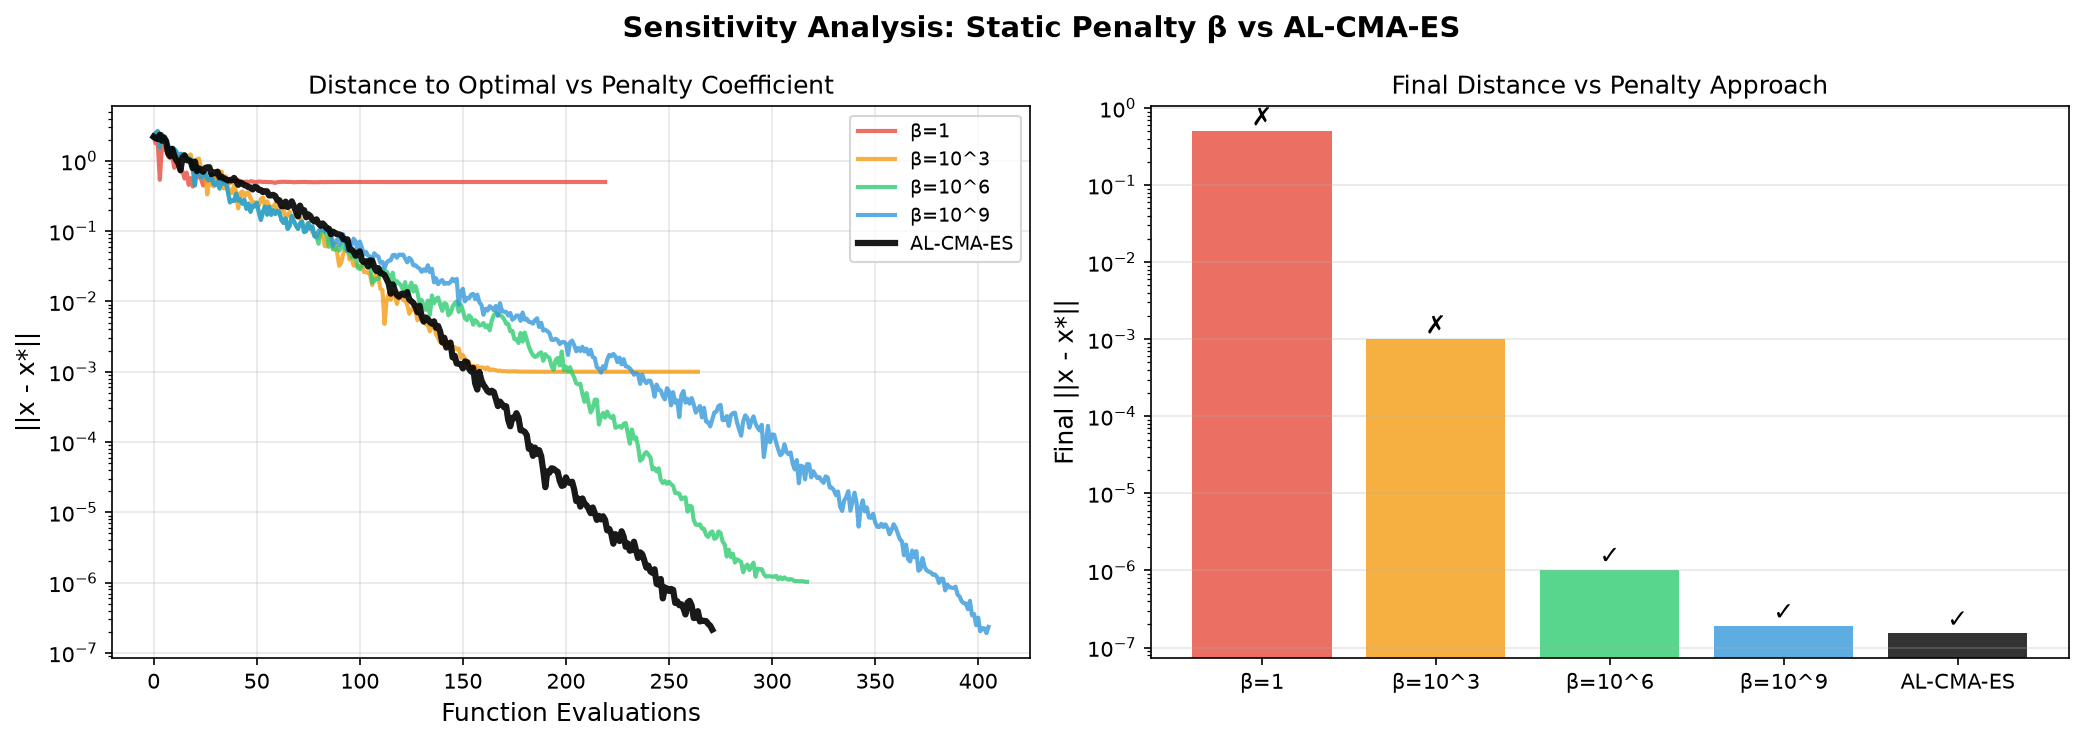
\includegraphics[width=0.92\linewidth]{results/alcmaes_comparison/part1_baseline/05_sensitivity_analysis.png}
  \caption{Linear constraint: penalty sensitivity.}
  \label{fig:exp-linear-sensitivity}
\end{figure}

\textbf{Adaptive penalty dynamics.}
The adaptive penalty method avoids selecting a single fixed $\beta$ by increasing the penalty coefficient when the search distribution remains infeasible. \Cref{fig:exp-linear-adaptive} illustrates this mechanism on a representative run: the distance to $\bm{x}^\star$ decreases steadily, while the penalty coefficient grows by many orders of magnitude (reaching $\beta\approx 10^{13}$ in this run) before feasibility is reliably enforced. This behavior explains why adaptive penalties can achieve feasibility without manual tuning on simple problems, yet may become numerically stiff: once $\beta$ is very large, the merit function is dominated by the constraint term, and further progress is governed by a near-feasibility regime that resembles a death-penalty behavior.

\begin{figure}[H]
  \centering
  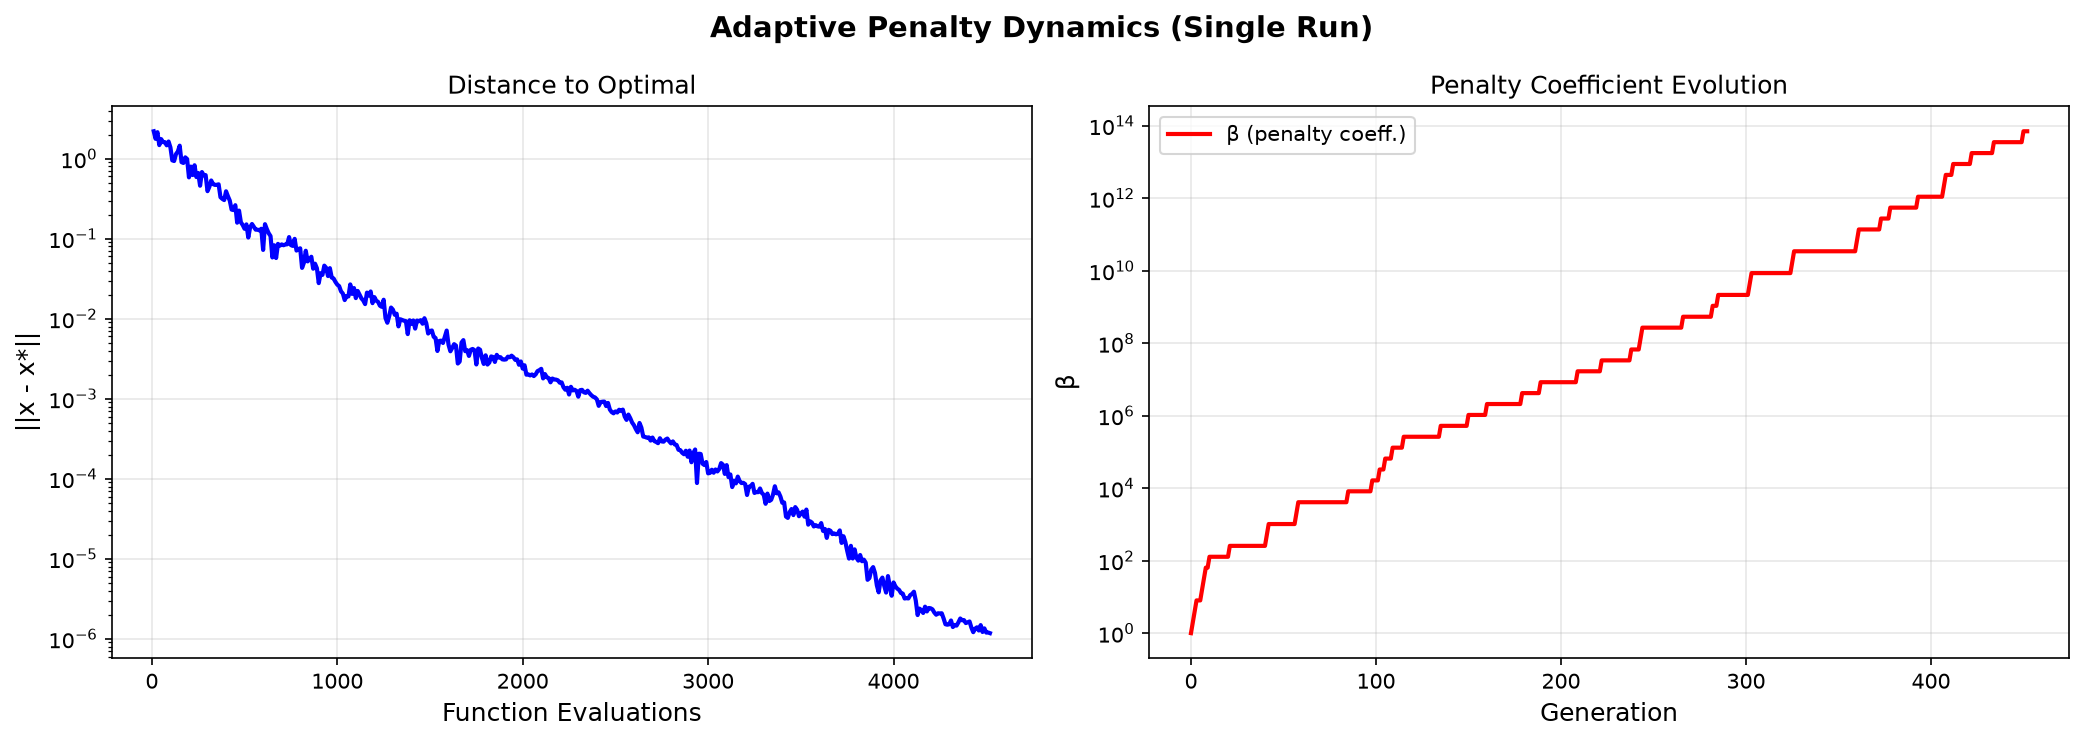
\includegraphics[width=0.92\linewidth]{results/alcmaes_comparison/part1_baseline/04_adaptive_dynamics.png}
  \caption{Linear constraint: adaptive penalty dynamics.}
  \label{fig:exp-linear-adaptive}
\end{figure}

\textbf{Internal behavior of AL-CMA-ES.}
To connect these outcomes to the internal state of the augmented Lagrangian mechanism, \cref{fig:exp-linear-internal} reports a representative run of AL-CMA-ES. The Lagrange multiplier converges toward $\gamma\approx 2$, matching the KKT value $\lambda^\star=2$ derived above, and then stabilizes. At the same time, the CMA-ES step-size $\sigma$ decreases steadily as the algorithm contracts around $\bm{x}^\star$, while the covariance condition number exhibits a transient increase before stabilizing. This pattern is consistent with a two-phase behavior in which the search first aligns with the constraint boundary and then refines the solution without requiring an extreme penalty coefficient.

\begin{figure}[H]
  \centering
  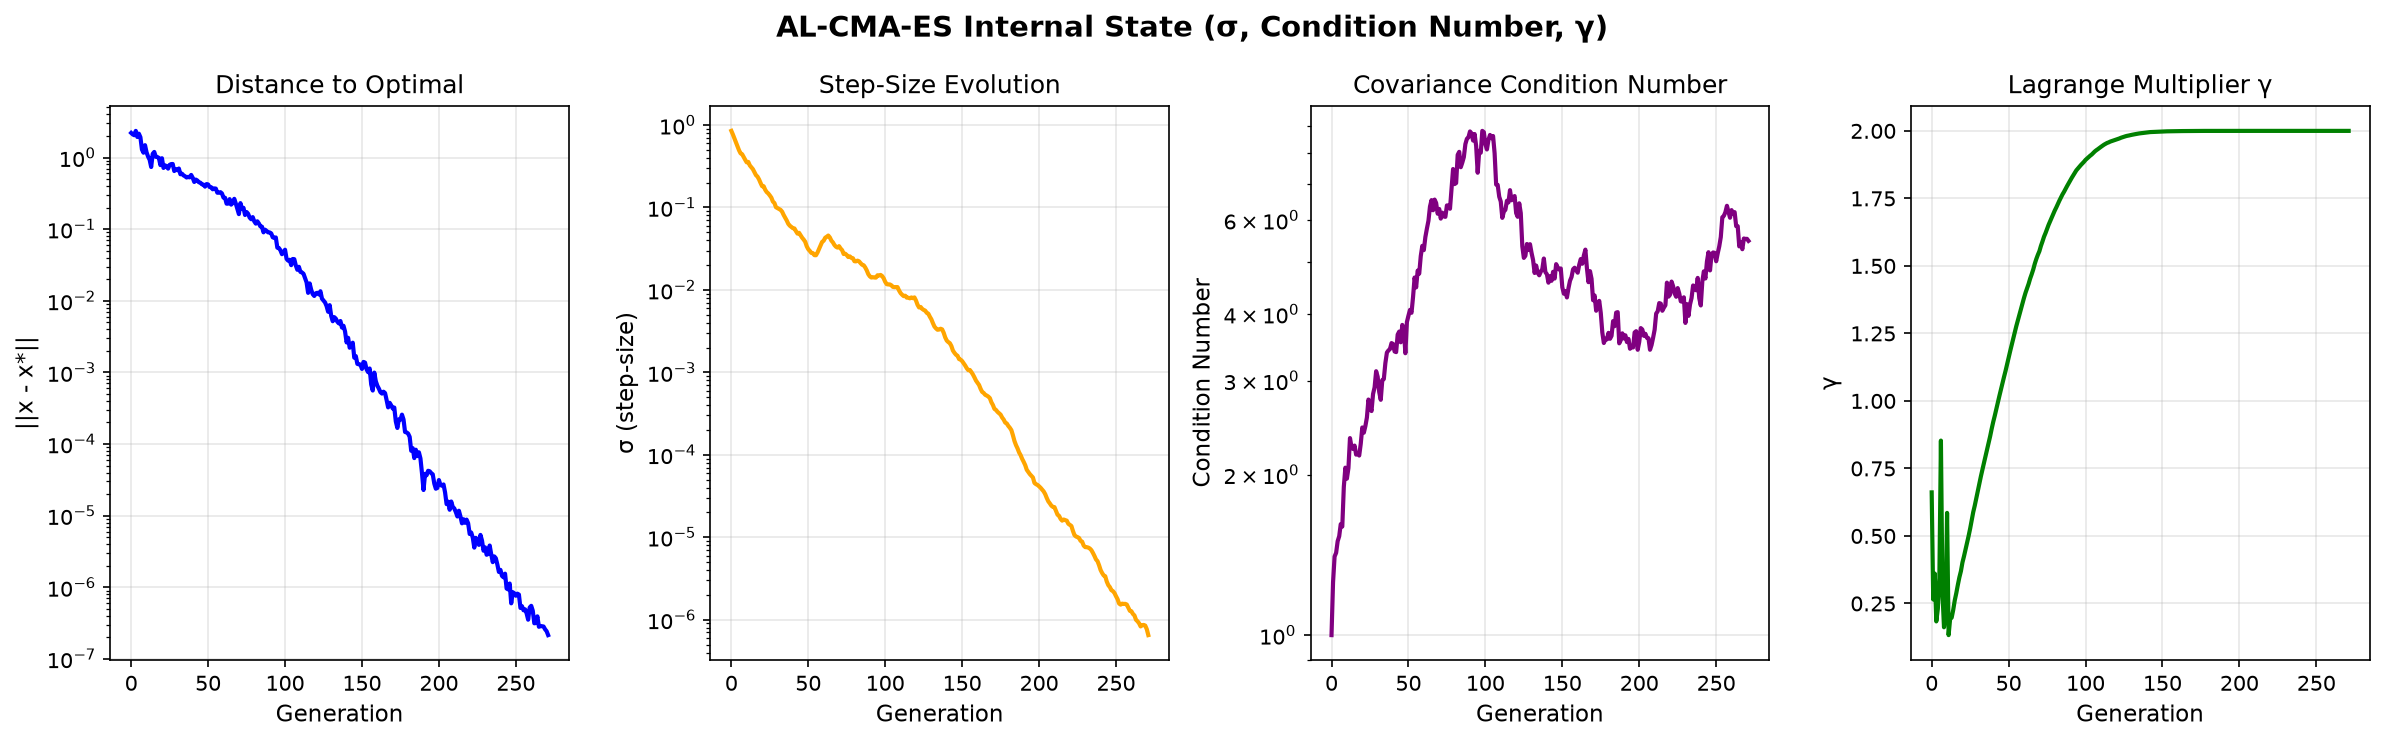
\includegraphics[width=0.98\linewidth]{results/alcmaes_comparison/part1_baseline/03_internal_state.png}
  \caption{Linear constraint: AL internal state.}
  \label{fig:exp-linear-internal}
\end{figure}

\subsubsection{Ill-conditioned ellipsoid benchmark}\label{subsubsec:exp-ill}
We next consider a single-constraint problem with a severely ill-conditioned objective. The objective is a convex ellipsoid with condition number $10^6$:
\begin{equation}
  \label{eq:ill-ellipsoid}
  \begin{aligned}
    \min_{\bm{x}\in\R^{10}}\quad &
    \sum_{i=1}^{10} 10^{6\frac{i-1}{9}}\,x_i^2,\\
    \text{s.t.}\quad & 10-x_1 \le 0.
  \end{aligned}
\end{equation}
With $g(\bm{x}) := 10-x_1$, the constrained optimum is $\bm{x}^\star=(10,0,\dots,0)$ and $f(\bm{x}^\star)=100$. All runs start from $\bm{x}^{(0)}=\bm{0}$ with $\sigma_0=5$ and are capped at 20\,000 evaluations. Since fixed-penalty methods are extremely sensitive to scaling on ill-conditioned objectives, we compare AL-CMA-ES to an adaptive quadratic penalty baseline.

\Cref{fig:exp-ill-convergence} shows the median distance to $\bm{x}^\star$ as a function of objective evaluations. Both methods exhibit an initial plateau, which is expected in ill-conditioned landscapes where the search distribution must first learn a strongly anisotropic covariance structure. After this adaptation phase, AL-CMA-ES reaches the high-accuracy regime earlier and terminates with fewer evaluations than the adaptive penalty scheme. The terminal statistics in \cref{tab:exp-ill-summary} confirm that both methods achieve feasibility in all runs under the adopted tolerance, while AL-CMA-ES reduces the median evaluation count by about 24\%.
\begin{table}[H]
  \centering
  \caption{Ill-conditioned ellipsoid: terminal statistics.}
  \label{tab:exp-ill-summary}
  \begin{tabular}{@{}l S[table-format=3.6] S[table-format=1.6] S[table-format=3.0] S[table-format=5.0]@{}}
    \toprule
    {Method} & {$f(\bm{x}_{\mathrm{final}})$} & {$g(\bm{x}_{\mathrm{final}})$} & {Feasible (\%)} & {FEvals} \\
    \midrule
    Adaptive Penalty & 100.000000 & 0.000000 & 100 & 7220 \\
    AL-CMA-ES & 100.000000 & 0.000000 & 100 & 5520 \\
    \bottomrule
  \end{tabular}
\end{table}

\begin{figure}[H]
  \centering
  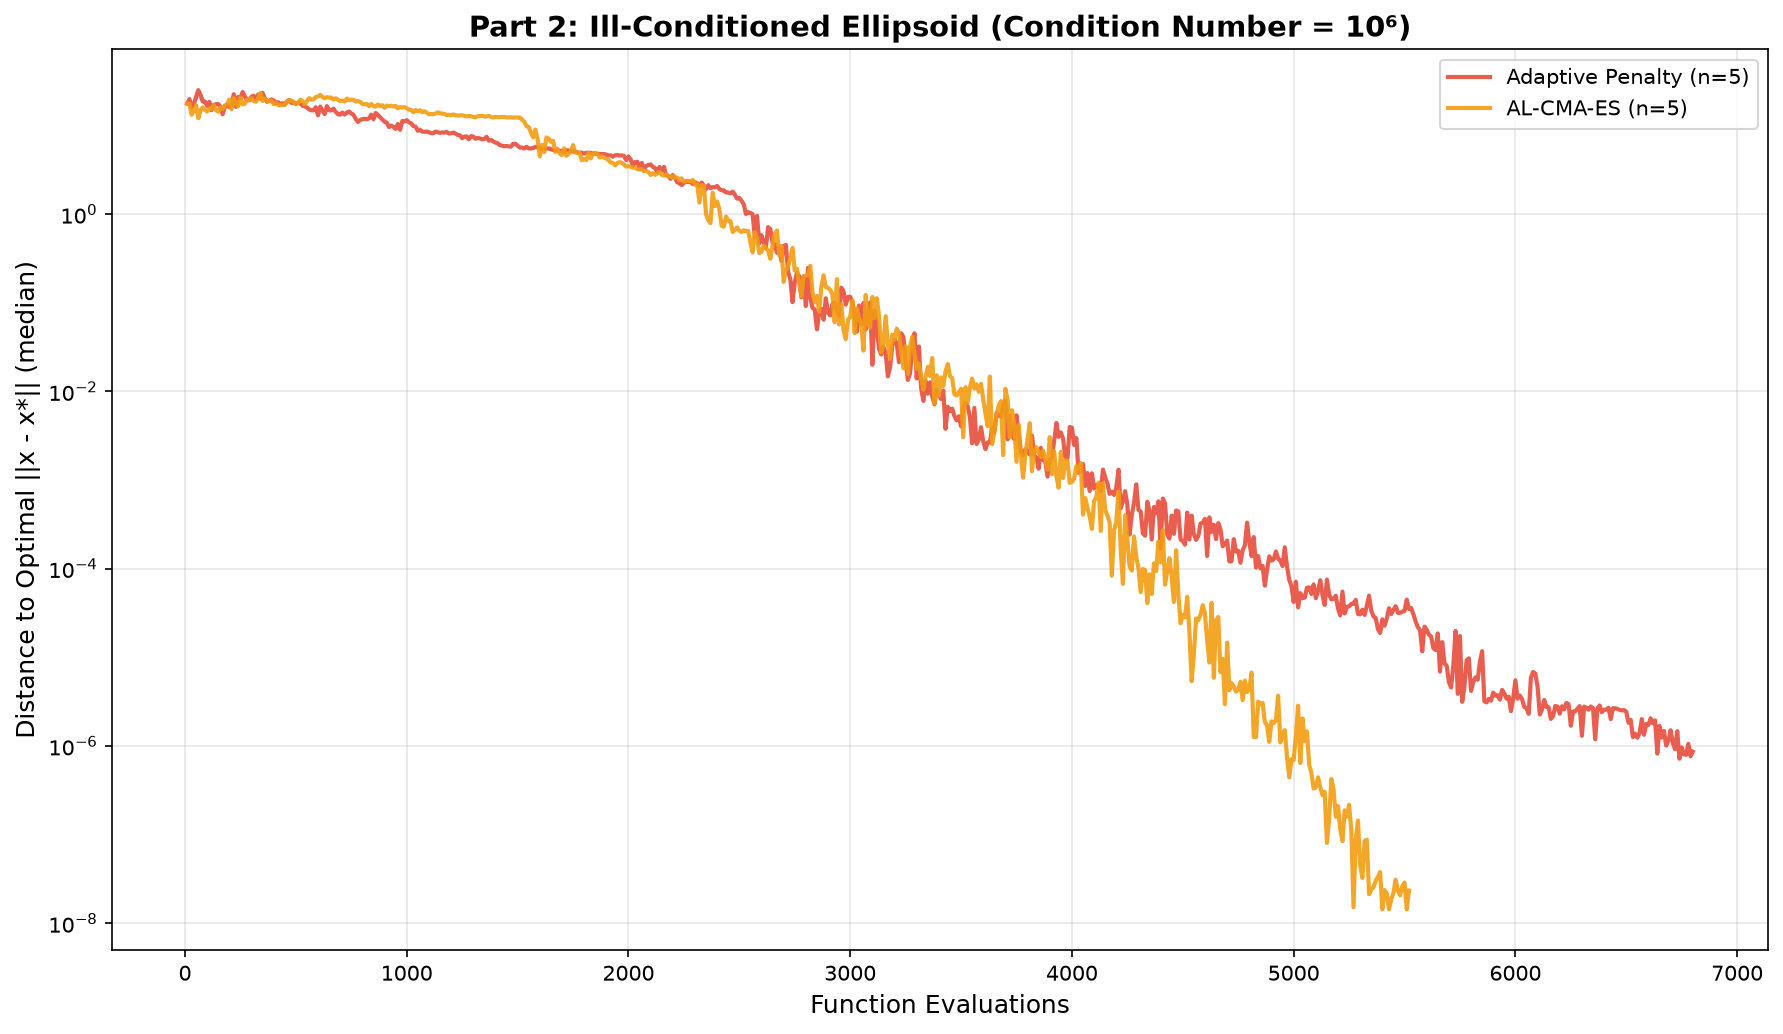
\includegraphics[width=0.92\linewidth]{results/alcmaes_comparison/part2_illconditioned/01_convergence_ellipsoid.png}
  \caption{Ill-conditioned ellipsoid: median convergence.}
  \label{fig:exp-ill-convergence}
\end{figure}




To relate this speed-up to the internal state of AL-CMA-ES, \cref{fig:exp-ill-internal} shows a representative run. 
\begin{figure}[H]
  \centering
  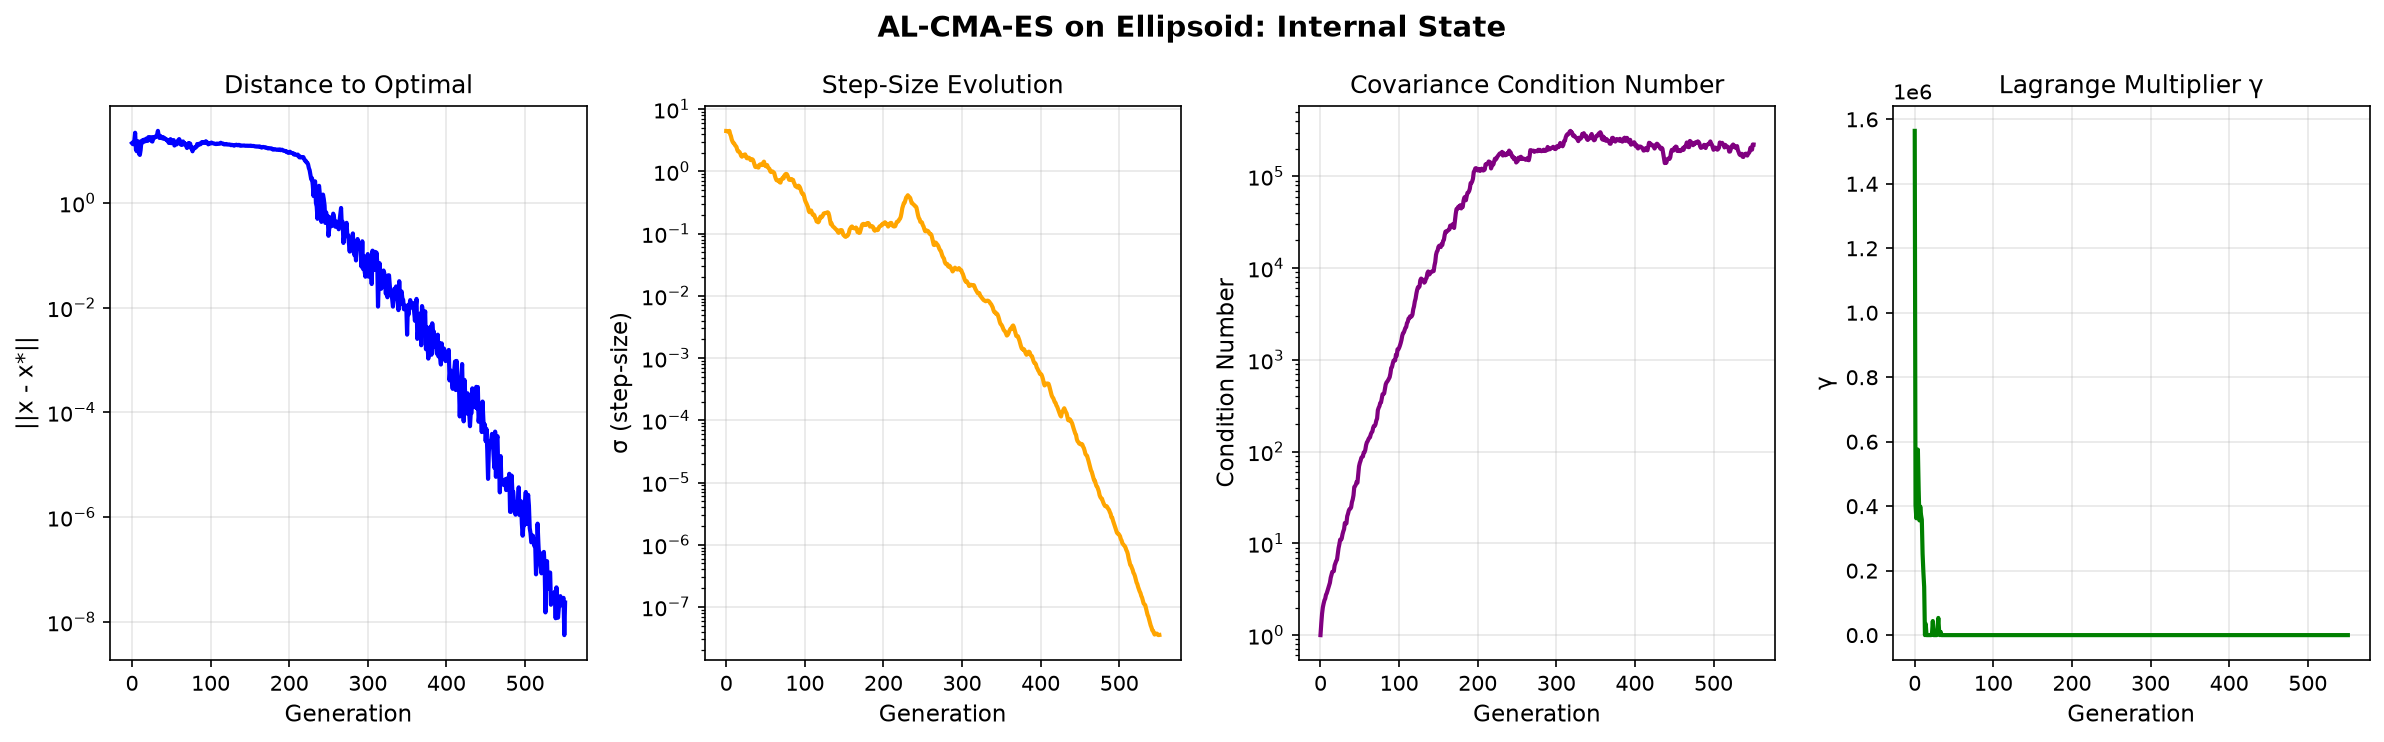
\includegraphics[width=0.98\linewidth]{results/alcmaes_comparison/part2_illconditioned/02_internal_state_al.png}
  \caption{Ill-conditioned ellipsoid: AL internal state.}
  \label{fig:exp-ill-internal}
\end{figure}
The step-size decreases steadily over several orders of magnitude, while the covariance condition number grows rapidly and then stabilizes, reflecting adaptation to the objective's anisotropy. The multiplier exhibits a sharp initial transient and then settles into comparatively small updates once the search distribution concentrates near the active boundary. This behavior is consistent with the AL mechanism enforcing feasibility early, while the remaining effort is dominated by covariance adaptation on an ill-conditioned landscape.

\subsubsection{Non-smooth constraint benchmark}\label{subsubsec:exp-nonsmooth}
The last scenario introduces a non-smooth inequality constraint with a gradient discontinuity at the boundary. The objective is a shifted sphere whose unconstrained minimizer lies in the infeasible region, while feasibility requires crossing a kink:
\begin{equation}
  \label{eq:nonsmooth}
  \begin{aligned}
    \min_{\bm{x}\in\R^{5}}\quad &
    (x_1-1)^2 + \sum_{i=2}^{5} x_i^2,\\
    \text{s.t.}\quad &
    g(\bm{x}) \le 0,\qquad
    g(\bm{x})=
    \begin{cases}
      2x_1, & x_1 \le 0,\\
      x_1, & x_1 > 0.
    \end{cases}
  \end{aligned}
\end{equation}
The feasible set is $\{x_1\le 0\}$ and the constrained optimum is $\bm{x}^\star=\bm{0}$ with $f(\bm{x}^\star)=1$. We initialize at $\bm{x}^{(0)}=0.5\,\bm{1}$ with $\sigma_0=0.5$ and use a budget of 10\,000 evaluations. \Cref{fig:exp-nonsmooth-constraint} visualizes the kink at $x_1=0$, which is known to induce oscillatory multiplier updates and to motivate surrogate or smoothing strategies in augmented Lagrangian schemes.\cite{DufosseHansen}

\begin{figure}[H]
  \centering
  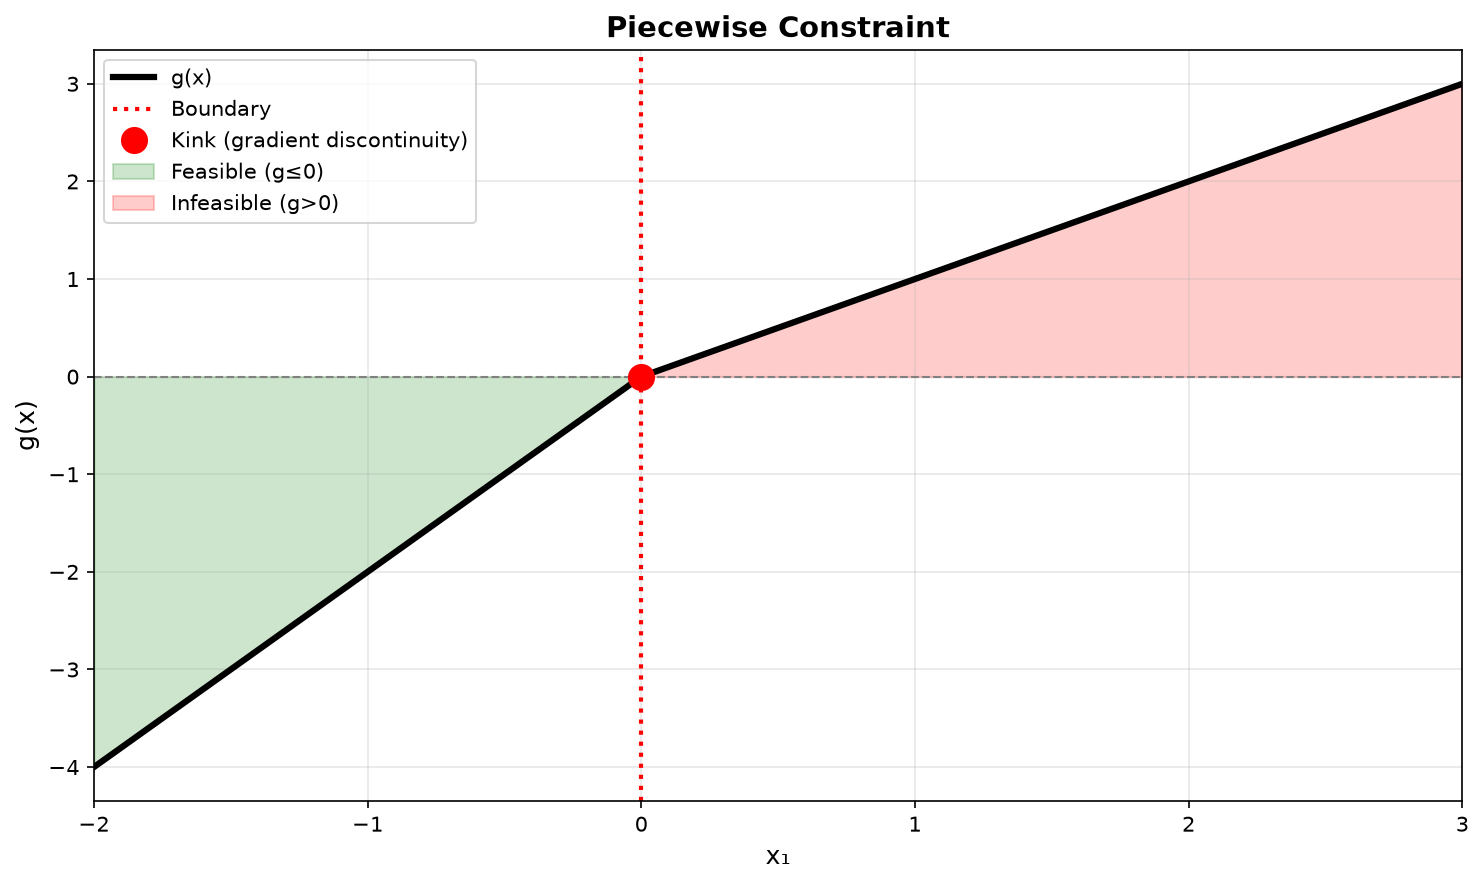
\includegraphics[width=0.86\linewidth]{results/alcmaes_comparison/part3_nonsmooth/02_constraint_function.png}
  \caption{Non-smooth constraint: kinked inequality.}
  \label{fig:exp-nonsmooth-constraint}
\end{figure}

We compare an adaptive penalty approach, standard AL-CMA-ES, and a surrogate-assisted AL variant. \Cref{fig:exp-nonsmooth-convergence} shows that the adaptive penalty decreases the distance to $\bm{x}^\star$ rapidly and terminates early in most runs, but does not reach 100\% feasibility under the adopted tolerance. Standard AL-CMA-ES progresses substantially more slowly, exhausts the evaluation budget in every run and is feasible in only three of the five runs: its final points oscillate across the kink, alternating between slightly infeasible points with objective values below $f(\bm{x}^\star)$ (drawn toward the infeasible unconstrained minimizer) and slightly feasible points just above it, which is where the median ends ($g=-1.0\times10^{-3}$, $f=1.0012$). The surrogate-assisted variant improves robustness, achieving 100\% feasibility and a steadily decreasing median distance, although it typically uses the full evaluation budget.

\begin{table}[H]
  \centering
  \caption{Non-smooth constraint: terminal statistics.}
  \label{tab:exp-nonsmooth-summary}
  \begin{tabular}{@{}l S[table-format=1.6] S[table-format=1.6] S[table-format=3.0] S[table-format=5.0]@{}}
    \toprule
    {Method} & {$f(\bm{x}_{\mathrm{final}})$} & {$g(\bm{x}_{\mathrm{final}})$} & {Feasible (\%)} & {FEvals} \\
    \midrule
    Adaptive Penalty & 1.000000 & 0.000000 & 60 & 1880 \\
    AL-CMA-ES & 1.001189 & -0.001009 & 60 & 10008 \\
    Surrogate-AL & 1.000000 & 0.000000 & 100 & 10008 \\
    \bottomrule
  \end{tabular}
\end{table}

\begin{figure}[H]
  \centering
  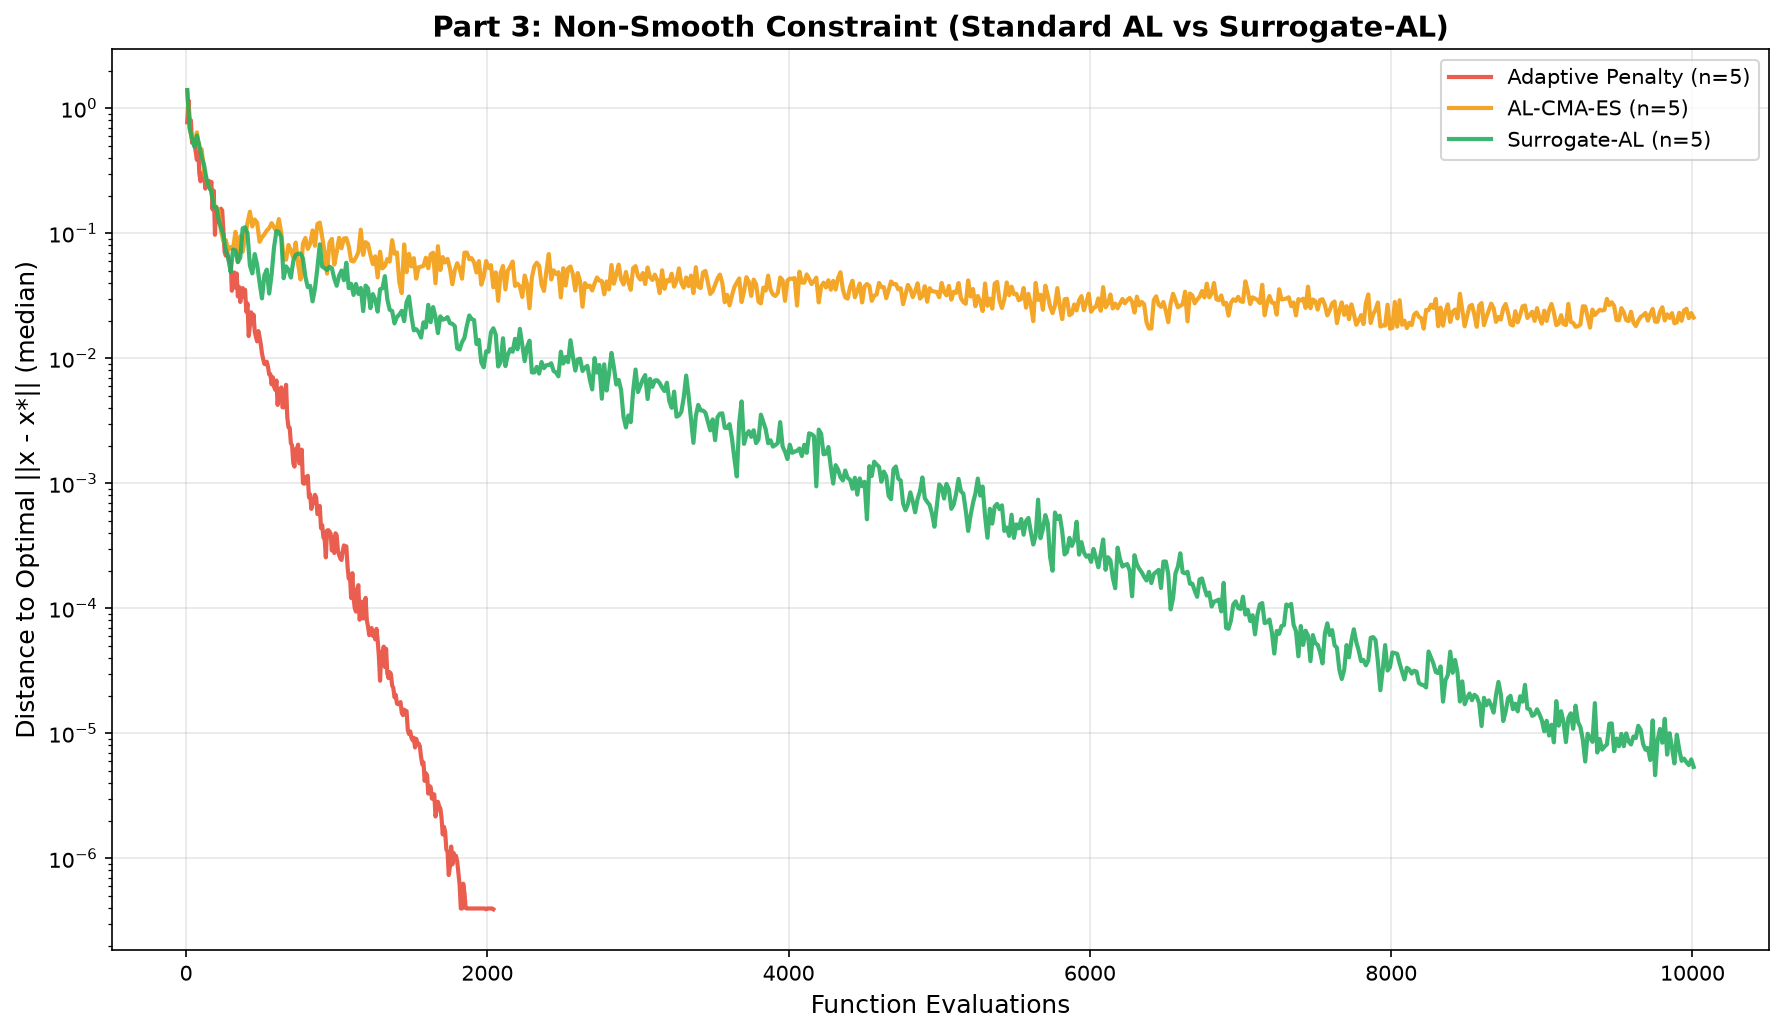
\includegraphics[width=0.92\linewidth]{results/alcmaes_comparison/part3_nonsmooth/01_convergence_nonsmooth.png}
  \caption{Non-smooth constraint: median convergence.}
  \label{fig:exp-nonsmooth-convergence}
\end{figure}

The multiplier trajectories in \cref{fig:exp-nonsmooth-gamma} highlight the effect of the kink. Because the left and right derivatives of $g$ differ at $x_1=0$, stationarity corresponds to a range of admissible multipliers rather than a single $\lambda^\star$, and the estimated $\gamma$ does not settle to one value. Both augmented Lagrangian variants keep $\gamma$ within the expected bounds. While Standard AL-CMA-ES exhibits irregular oscillations associated with slight infeasibility, the Surrogate-AL variant displays high-frequency, full-amplitude oscillations (see \cref{fig:exp-nonsmooth-gamma}). This indicates that the surrogate model effectively maintains the search tightly along the non-smooth boundary, preventing the drift into the infeasible region observed in the standard approach.

\begin{figure}[H]
  \centering
  \begin{subfigure}[b]{0.49\linewidth}
    \centering
    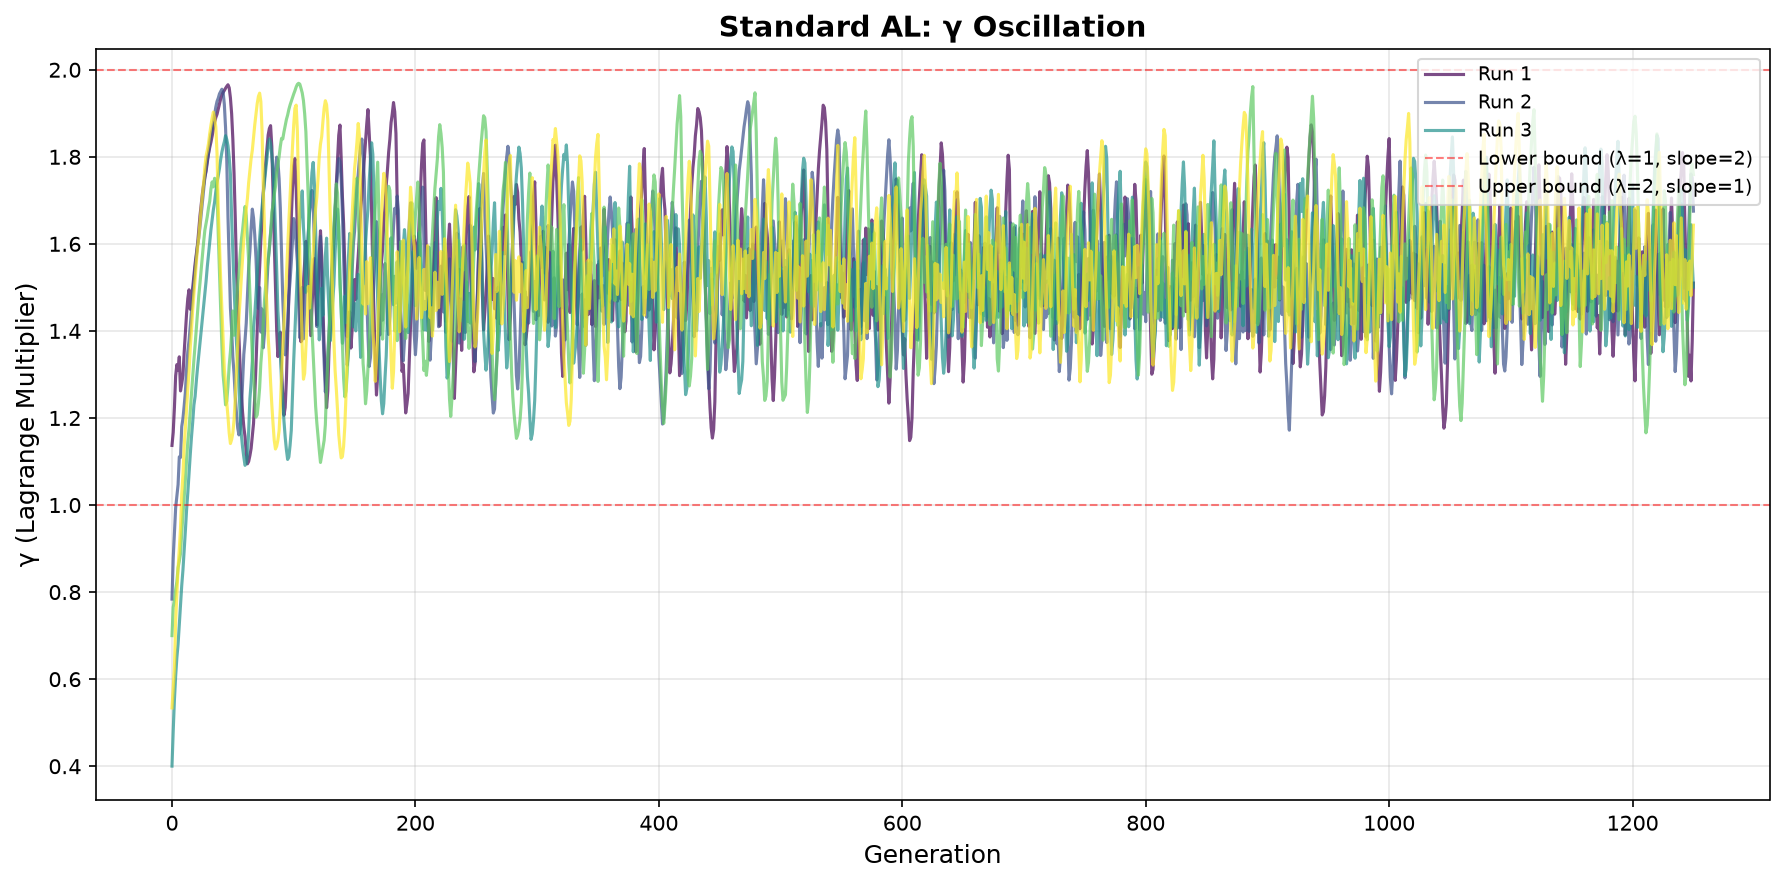
\includegraphics[width=\linewidth]{results/alcmaes_comparison/part3_nonsmooth/03_gamma_oscillation_al.png}
    \caption{Standard AL.}
  \end{subfigure}
  \hfill
  \begin{subfigure}[b]{0.49\linewidth}
    \centering
    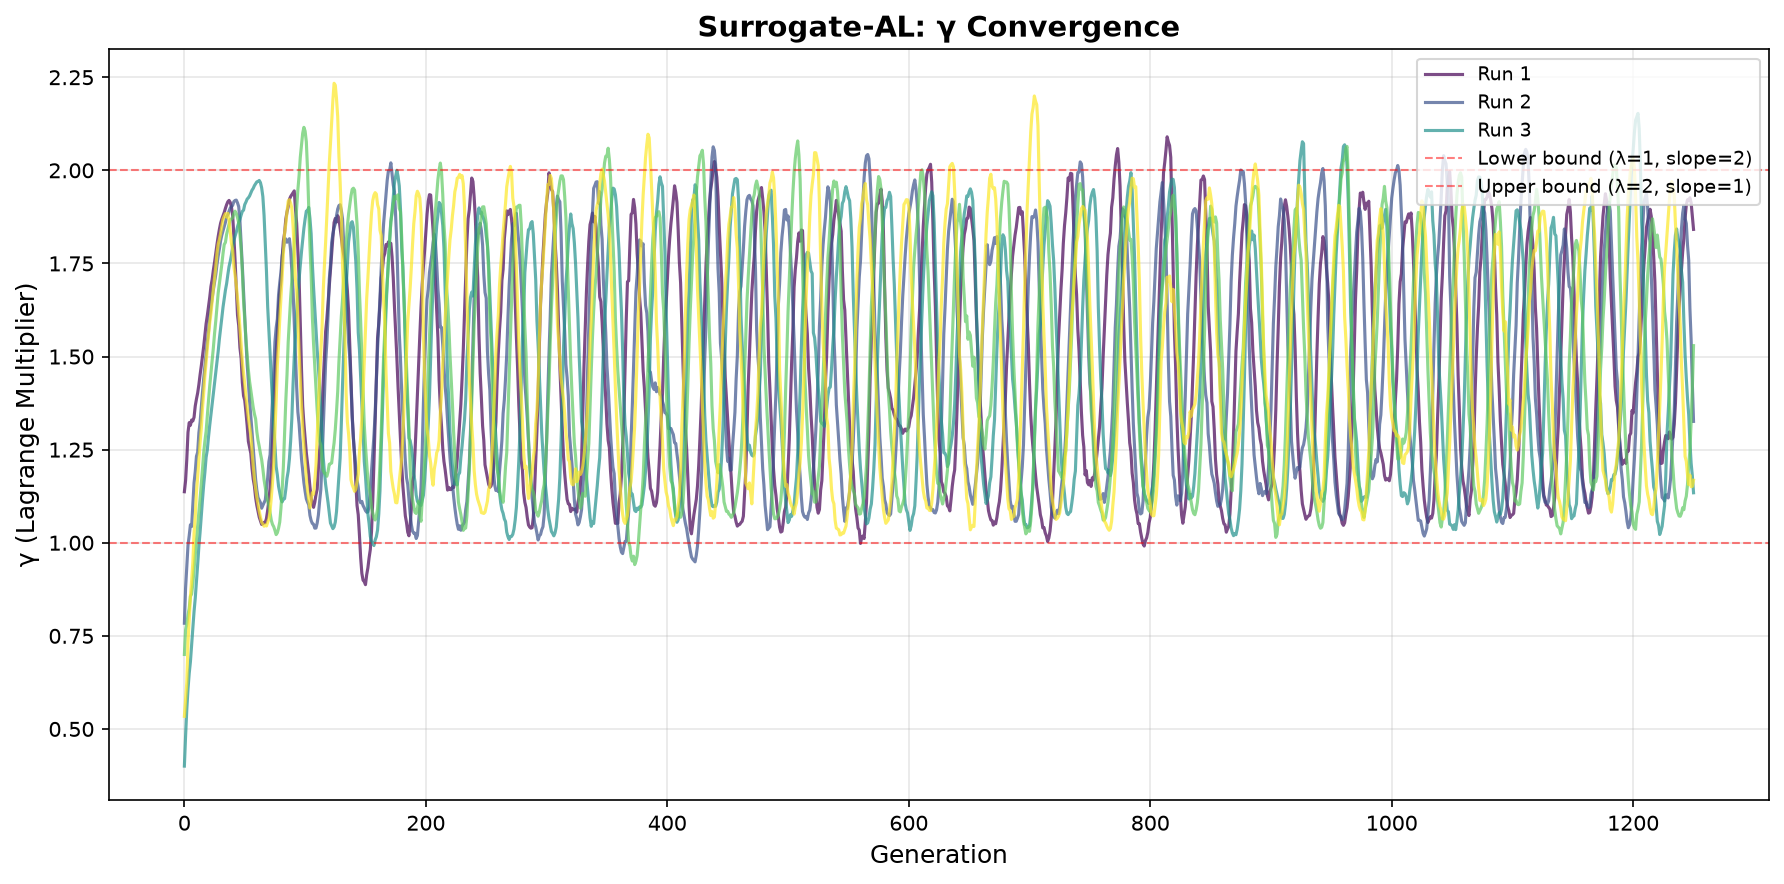
\includegraphics[width=\linewidth]{results/alcmaes_comparison/part3_nonsmooth/04_gamma_surrogate.png}
    \caption{Surrogate-AL.}
  \end{subfigure}
  \caption{Non-smooth constraint: multiplier dynamics.}
  \label{fig:exp-nonsmooth-gamma}
\end{figure}

Across the three scenarios, AL-CMA-ES consistently balances objective progress and feasibility without relying on extreme fixed penalties. On the linear benchmark it attains the constrained solution with fewer evaluations than death and adaptive penalties, and it avoids the tuning sensitivity of static penalties. On the ill-conditioned ellipsoid, it remains competitive and improves efficiency relative to adaptive penalties while the covariance adapts to anisotropy. For non-smooth constraints, however, multiplier oscillations can dominate and motivate surrogate or smoothing strategies when strong feasibility reliability is required.


% ============================================================
\section{Summary and Discussion}\label{sec:summary}

In this work, we analyzed the integration of the Augmented Lagrangian method into the CMA-ES framework, addressing the limitations of static and simple adaptive penalty functions in constrained black-box optimization. By formalizing the algorithm as an interaction between the primal evolutionary search and a dual update scheme, we demonstrated that AL-CMA-ES provides a principled mechanism to enforce feasibility without compromising the conditioning of the underlying objective landscape.

Our theoretical analysis and numerical experiments support the following conclusions regarding the efficacy and behavior of the method:

\begin{itemize}
    \item \textbf{Decoupling Feasibility from Conditioning:} 
    The primary advantage of the Augmented Lagrangian over quadratic penalty methods is the separation of concerns. By using the Lagrange multipliers ($\gamma$) to provide a first-order shift of the stationary point, the algorithm reduces the reliance on the penalty parameter ($\omega$). This prevents the formation of pathological, narrow valleys associated with large penalty coefficients, allowing the CMA-ES covariance adaptation to function effectively even on ill-conditioned problems.

    \item \textbf{Sample Efficiency vs. Baselines:} 
    On the linear constraint benchmark, AL-CMA-ES demonstrated superior sample efficiency compared to the Death Penalty and Adaptive Penalty methods. Unlike the Death Penalty, which discards information from infeasible samples, the AL formulation utilizes the gradient of the constraint violation to guide the mean toward the feasible region actively. Unlike static penalties, it avoids the stagnation caused by insufficient penalty weights and the numerical stiffness caused by excessive ones.

    \item \textbf{Robustness to Objective Scaling:} 
    The experiments on the ill-conditioned ellipsoid confirmed that the internal adaptation of the augmented Lagrangian parameters does not interfere with the covariance matrix adaptation of CMA-ES. The method successfully learned the high-aspect-ratio scaling of the objective while simultaneously satisfying the constraint, a scenario where static penalty methods typically fail due to the inability to balance the penalty magnitude against the objective's steep gradients.

    \item \textbf{Limitations on Non-smooth Constraints:} 
    The non-smooth benchmark highlighted a boundary condition for the method's reliability. The discontinuity in the constraint gradient led to oscillations in the multiplier updates, preventing the standard AL-CMA-ES from stabilizing strictly on the feasible side of the boundary. This suggests that while the method is robust for smooth constraints (even with ill-conditioned objectives), problems with non-smooth or noisy constraint boundaries may require surrogate-assisted variants or smoothing techniques to dampen dual oscillations.
\end{itemize}

In conclusion, AL-CMA-ES represents a robust default strategy for constrained continuous optimization. It eliminates the need for problem-specific parameter tuning inherent in static penalty methods and provides a more informative search landscape than rejection-based strategies.

\clearpage
\begin{thebibliography}{9}

\bibitem{Atamna2016}
A.~Atamna, A.~Auger, and N.~Hansen,
\newblock ``Augmented Lagrangian Constraint Handling for CMA-ES---Case of a Single Linear Constraint,''
\newblock in \emph{Proceedings of the 2016 Genetic and Evolutionary Computation Conference (GECCO)}, 2016.

\bibitem{Atamna2017}
A.~Atamna, A.~Auger, and N.~Hansen,
\newblock ``Linearly Convergent Evolution Strategies via Augmented Lagrangian Constraint Handling,''
\newblock in \emph{Proceedings of the 14th ACM/SIGEVO Conference on Foundations of Genetic Algorithms (FOGA)}, 2017.

\bibitem{ArnoldPorter2015}
D.~V.~Arnold and J.~Porter,
\newblock ``Towards an Augmented Lagrangian Constraint Handling Approach for the (1+1)-ES,''
\newblock in \emph{Proceedings of the 2015 Genetic and Evolutionary Computation Conference (GECCO)}, 2015.

\bibitem{NocedalWright}
J.~Nocedal and S.~J.~Wright,
\newblock \emph{Numerical Optimization},
\newblock 2nd ed., Springer, 2006.

\bibitem{DufosseHansen}
P.~Dufoss{\'e} and N.~Hansen,
\newblock ``Augmented Lagrangian, penalty techniques and surrogate modeling for constrained optimization with CMA-ES,''
\newblock in \emph{Proceedings of the Genetic and Evolutionary Computation Conference (GECCO)}, 2021.

\end{thebibliography}

\end{document}